\documentclass[sigplan,10pt]{acmart}

\usepackage{amsmath}
\usepackage{enumitem}
\usepackage{xspace}
\usepackage{caption}
\usepackage{subcaption}
\usepackage{float}
\usepackage{cleveref}
\usepackage[small, compact]{titlesec}
\newcommand{\tech}[0]{PagedAttention\xspace}
\newcommand{\sys}[0]{vLLM\xspace}

% \renewcommand\footnotetextcopyrightpermission[1]{}
\settopmatter{printacmref=false, printccs=true, printfolios=true}
\newcommand{\heading}[1]{\vspace{4pt}\noindent\textbf{#1}}
\newcommand{\topheading}[1]{\noindent\textbf{#1}}

% Compact itemize and enumerate.
\usepackage{enumitem}
\newenvironment{CompactItemize}
  {\begin{itemize}[noitemsep,topsep=0pt,leftmargin=*]}
  {\end{itemize}}
\newenvironment{CompactEnumerate}
  {\begin{enumerate}[noitemsep,topsep=0pt,leftmargin=*]}
  {\end{enumerate}}

\newcommand{\plainauthors}{Woosuk Kwon, Zhuohan Li, Siyuan Zhuang, Ying Sheng, Lianmin Zheng, Cody Hao Yu, Joseph E. Gonzalez, Hao Zhang, Ion Stoica}
\renewcommand{\shortauthors}{Woosuk Kwon et al.}

\setcopyright{rightsretained}

\begin{document}

\title{Efficient Memory Management for Large Language Model Serving with \emph{PagedAttention}}

\author{Woosuk Kwon$^{\text{1}, *}$\enskip Zhuohan Li$^{\text{1}, *}$\enskip Siyuan Zhuang$^{\text{1}}$\enskip Ying Sheng$^{\text{1}, \text{2}}$\enskip Lianmin Zheng$^{\text{1}}$\enskip Cody Hao Yu$^{\text{3}}$\enskip \\ Joseph E. Gonzalez$^{\text{1}}$\enskip Hao Zhang$^{\text{4}}$\enskip Ion Stoica$^{\text{1}}$}
\affiliation{\vspace{1mm} $^{\text{1}}$UC Berkeley \enskip $^{\text{2}}$Stanford University \enskip $^{\text{3}}$Independent Researcher \enskip $^{\text{4}}$UC San Diego \country{}}

\begin{abstract}
High throughput serving of large language models (LLMs) requires batching sufficiently many requests at a time.
However, existing systems struggle because the key-value cache (KV cache) memory for each request is huge and grows and shrinks dynamically.
When managed inefficiently, this memory can be significantly wasted by fragmentation and redundant duplication, limiting the batch size.
To address this problem, we propose \tech, an attention algorithm inspired by the classical virtual memory and paging techniques in operating systems.
On top of it, we build \sys, an LLM serving system that achieves (1) near-zero waste in KV cache memory and (2) flexible sharing of KV cache within and across requests to further reduce memory usage.
Our evaluations show that \sys improves the throughput of popular LLMs by 2-4$\times$ with the same level of latency compared to the state-of-the-art systems, such as FasterTransformer and Orca.
The improvement is more pronounced with longer sequences, larger models, and more complex decoding algorithms.
\sys's source code is publicly available at~\url{https://github.com/vllm-project/vllm}.
\end{abstract}


\acmYear{2023}\copyrightyear{2023}
\acmConference[SOSP '23]{ACM SIGOPS 29th Symposium on Operating Systems Principles}{October 23--26, 2023}{Koblenz, Germany}
\acmBooktitle{ACM SIGOPS 29th Symposium on Operating Systems Principles (SOSP '23), October 23--26, 2023, Koblenz, Germany}
\acmPrice{}
\acmDOI{10.1145/3600006.3613165}
\acmISBN{979-8-4007-0229-7/23/10}

\maketitle
\pagestyle{plain}

\section{Introduction}
\label{sec:intro}


Transformers, in particular decoder-only models (e.g.\ GPT~\citep{brown2020language}, Llama~\citep{touvron2023llama}) which process input sequences in a causal fashion, are one of the main drivers of modern deep learning's success.
Numerous approaches attempt to approximate the core attention layer to address its efficiency issues~\citep{tay2022efficient}, such as scaling quadratically in sequence length during training and requiring a cache of size linear in sequence length during autoregressive generation.
In parallel, a class of alternative sequence models, structured state-space models (SSMs), have emerged with linear scaling in sequence length during training and constant state size during generation.
They show strong performance on long-range tasks (e.g. S4~\citep{gu2022efficiently}) and recently matched or beat Transformers on language modeling (e.g. Mamba \citep{gu2023mamba}) at small to moderate scale.
However, the development of SSMs have appeared disjoint from the community's collective effort to improve Transformers, such as understanding them theoretically as well as optimizing them on modern hardware.
As a result, it is more difficult to understand and experiment with SSMs compared to Transformers, and it remains challenging to train SSMs as efficiently as Transformers from both an algorithmic and systems perspective.


Our main goal is to develop a rich body of theoretical connections between structured SSMs and variants of attention.
This will allow us to transfer algorithmic and systems optimizations originally developed for Transformers to SSMs, towards the goal of building foundation models that perform better than Transformers while scaling more efficiently in sequence length.
A milestone contribution in this direction was the \textbf{Linear Attention (LA)} framework \citep{katharopoulos2020transformers},
which derived a connection between autoregressive attention and linear RNNs
by showing the equivalence between ``dual forms'' of quadratic kernelized attention and a particular linear recurrence.
This duality allows new capabilities such as the ability to have both efficient parallelizable training and efficient autoregressive inference.
In the same spirit, this paper provides multiple viewpoints connecting linear-complexity SSMs with quadratic-complexity forms to combine the strengths of SSMs and attention.%
\footnote{Technically speaking, these connections only relate to certain flavors of attention; the title of this paper is an homage to \citet{katharopoulos2020transformers} which first showed that ``Transformers are RNNs''.}

\iftoggle{arxiv}{
\begin{wrapfigure}{R}{0.48\linewidth}
  \begin{center}
    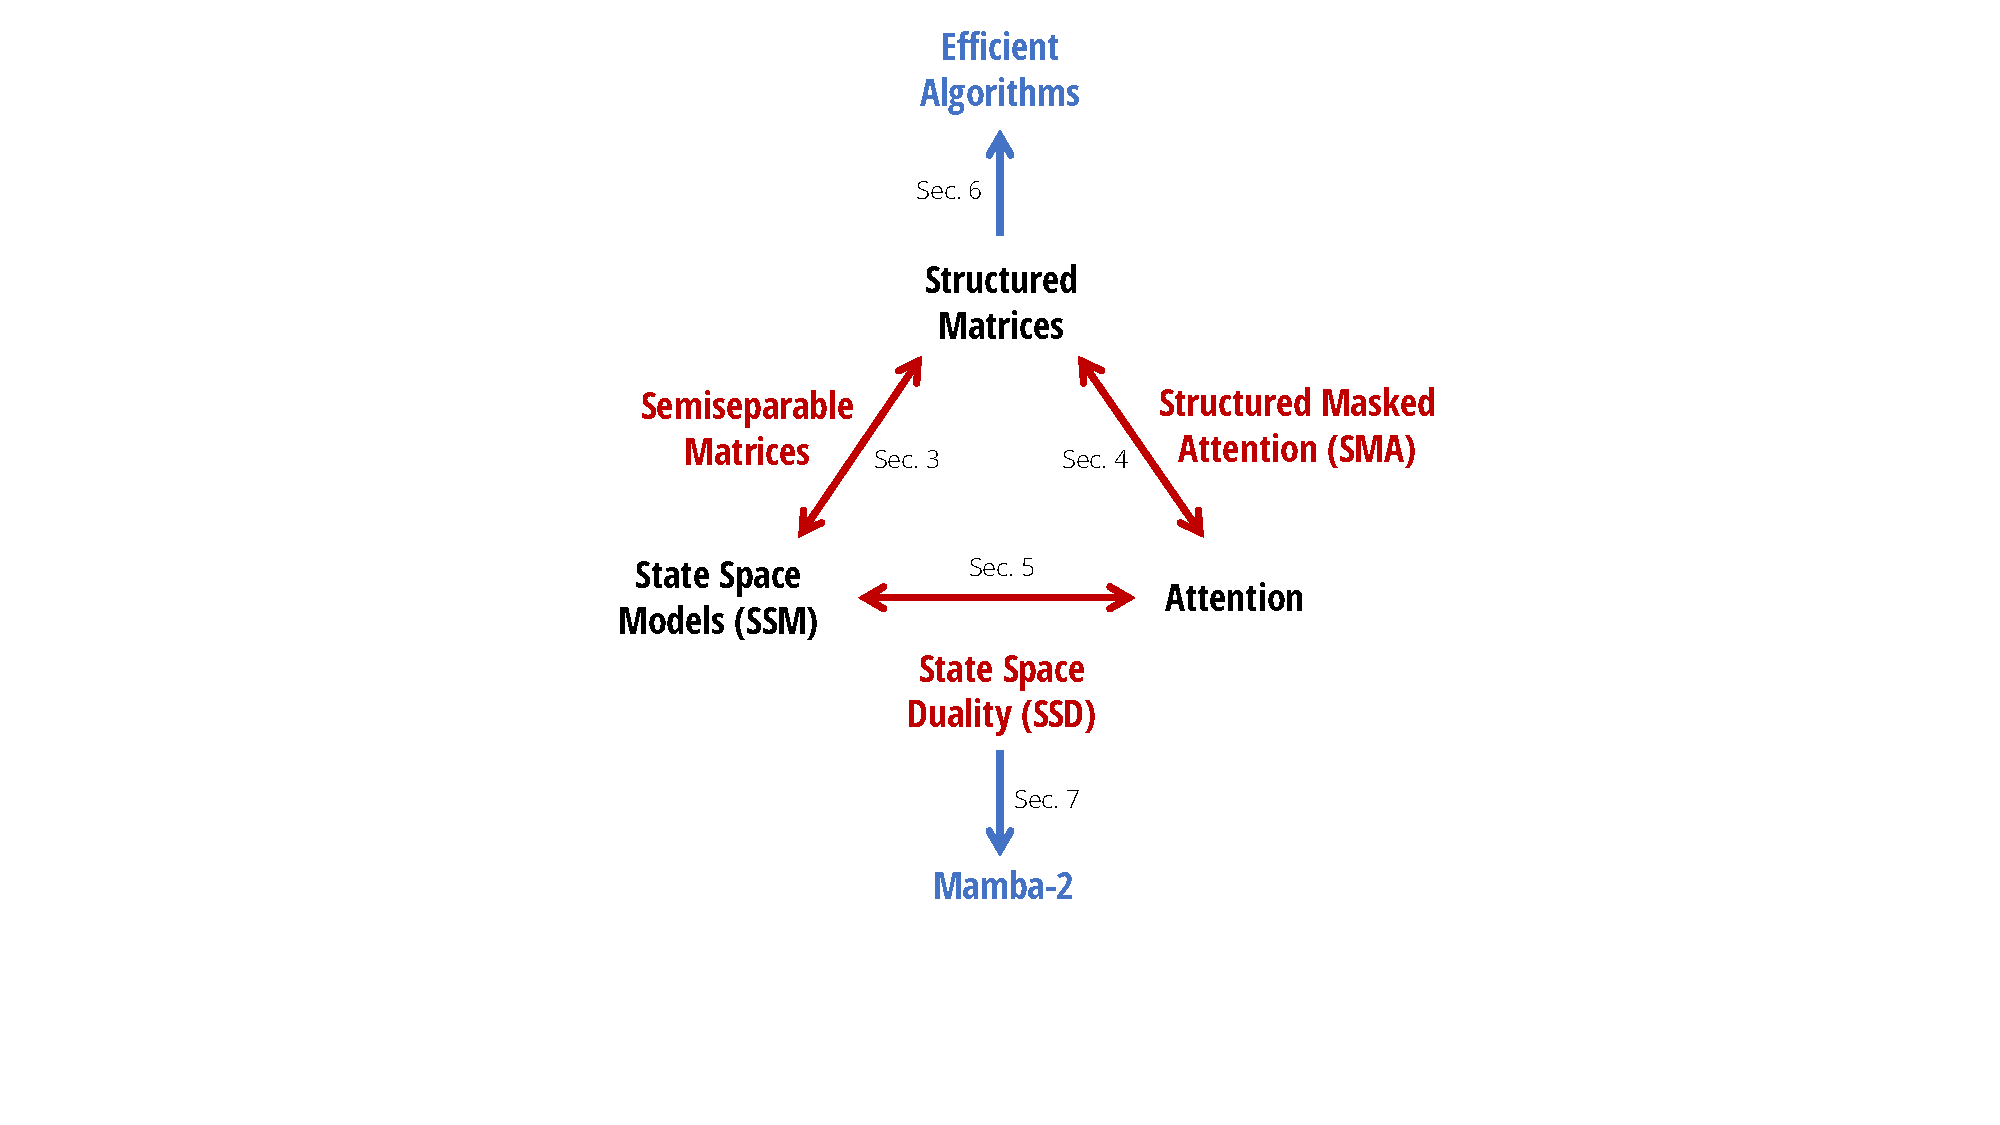
\includegraphics[width=\linewidth]{fig/ssd_roadmap.pdf}
  \end{center}
  \caption{
    (\textbf{Structured State-Space Duality}.)
    This paper fleshes out the relationship between state space models and attention through the bridge of structured matrices.
  }
  \label{fig:roadmap}
\end{wrapfigure}
}{}

\para{State Space Duality.}
Our framework connecting structured SSMs and variants of attention, which we call \textbf{structured state space duality} (SSD),
is made through the abstractions of \textbf{structured matrices}:
matrices with subquadratic parameters and multiplication complexity.
We develop two broad frameworks for representing sequence models, one as matrix transformations and one as tensor contractions, which each reveal different perspectives of the duality.
Our technical contributions include:
\begin{itemize}[leftmargin=*,itemsep=0pt,topsep=0pt]
  \item We show an equivalence between state space models and a well-studied family of structured matrices called \textbf{semiseparable matrices}\iftoggle{arxiv}{ (\cref{sec:ssm})}{}.
    This connection is at the heart our framework, revealing new properties and algorithms for SSMs. A central message of this paper is that \emph{different methods of computing state space models can be reframed as various matrix multiplication algorithms on structured matrices}.
  \item We significantly improve the theory of linear attention~\citep{katharopoulos2020transformers}.
    We first provide an incisive proof of its recurrent form through the language of tensor contractions, and then generalize it to a new family of \textbf{structured masked attention (SMA)}\iftoggle{arxiv}{ (\cref{sec:attention})}{}.
  \item We connect SSMs and SMA, showing that they have a large intersection that are duals of each other, possessing both SSM-like linear and attention-like quadratic forms\iftoggle{arxiv}{ (\cref{sec:ssd})}{}.
    \iftoggle{arxiv}{We also prove that any kernel attention method possessing a fast recurrent form must be an SSM.}{}
\end{itemize}


Beyond its intrinsic theoretical value, our framework opens up a broad set of directions for understanding and improving sequence models.

\para{Efficient Algorithms.}
First and most importantly, our framework exposes new efficient and easily-implementable algorithms for computing SSMs\iftoggle{arxiv}{ (\cref{sec:efficient})}{}.
We introduce a new \textbf{SSD algorithm}, based on block decompositions of semiseparable matrices, that takes advantage of both the linear SSM recurrence and quadratic dual form, obtaining optimal tradeoffs on all main efficiency axes (e.g. training and inference compute, memory usage, and ability to leverage matrix multiplication units on modern hardware).
A dedicated implementation of SSD is $2-8\times$ faster than the optimized selective scan implementation of Mamba, while simultaneously allowing for much larger recurrent state sizes ($8\times$ the size of Mamba or even higher, with minimal slowdown).
SSD is highly competitive with optimized implementations of softmax attention (FlashAttention-2~\citep{dao2023flashattention2}), crossing over at sequence length 2K and 6$\times$ faster at sequence length 16K.


\iftoggle{arxiv}{
\para{Architecture Design.}
One major obstacle to adopting new architectures such as SSMs is the ecosystem tailored to Transformers, such as hardware-efficient optimization and parallelism techniques for large-scale training.
Our framework allows using established conventions and techniques for attention to build a vocabulary of architecture design choices for SSMs, and further improve them (\cref{sec:architecture}).
For example, we introduce the analog of heads from multi-head attention (MHA) to SSMs.
We show that the Mamba architecture is a \textbf{multi-input SSM (MIS)} that turns out to be analogous to \textbf{multi-value attention (MVA)}, and compare other variants of Mamba with different head structures.

We also use these ideas to make slight modifications to the Mamba block, which allows tensor parallelism to be implemented (e.g. in the style of Megatron~\citep{shoeybi2019megatron}).
The main ideas include introducing grouped-value attention (GVA) head structure, and moving all data-dependent projections to occur in parallel at the beginning of the block.


}{
  \para{Mamba-2.}
  Additionally, inspired by the connection between SSMs and Transformers, we slightly modify the neural network architecture of Mamba by moving all data-dependent projections to occur in parallel at the beginning of the block. %
}
The combination of the modified parallel Mamba block, together with using SSD as the inner SSM layer, results in the \textbf{Mamba-2} architecture.
We investigate Chinchilla scaling laws for Mamba-2 in the same setting as Mamba, finding that it Pareto dominates Mamba and Transformer++ in both perplexity and wall-clock time.
We additionally train a family of Mamba-2 models at varying sizes on the Pile, showing that it matches or outperforms Mamba and open source Transformers on standard downstream evaluations.
For example, Mamba-2 with 2.7B parameters trained on 300B tokens on the Pile outperforms Mamba-2.8B, Pythia-2.8B and even Pythia-6.9B trained on the same dataset.

\iftoggle{arxiv}{
\paragraph{Systems Optimizations.}
The SSD framework connects SSMs and Transformers, allowing us to leverage a rich body of work on systems optimizations developed for Transformers~(\cref{sec:systems}).
\begin{itemize}[leftmargin=*,itemsep=0pt,topsep=0pt]
  \item For example, Tensor Parallelism (TP) is an important model parallelism technique to train large Transformer models by splitting each layer across GPUs on the same node.
    We design Mamba-2 to be TP-friendly, reducing the number of synchronization point per block by half.
  \item For very long sequences whose activations do not fit on one device, sequence parallelism has been developed for the attention blocks.
    We describe how to train SSMs in general and Mamba-2 in particular with sequence parallelism, by passing the recurrent states between devices.
  \item For finetuning with examples of different lengths, for best efficiency, Transformer requires sophisticated techniques to remove padding tokens and perform attention on variable length sequences.
    We show how Mamba-2 can be trained with variable sequence lengths efficiently, requiring no padding tokens.
\end{itemize}
}{}

\cref{sec:experiments} empirically validates Mamba-2 on language modeling, training efficiency, and a difficult multi-query associative recall task~\citep{arora2024simple}.
Finally, in \cref{sec:related}, we provide an extended related work and discuss potential research directions opened up by our framework.

Model code and pre-trained checkpoints are open-sourced at \url{https://github.com/state-spaces/mamba}.







\section{Background}

In this section, we describe the generation and serving procedures of typical LLMs and the iteration-level scheduling used in LLM serving.

\subsection{Transformer-Based Large Language Models}
The task of language modeling is to model the probability of a list of tokens $(x_1, \ldots, x_n).$ Since language has a natural sequential ordering, it is common to factorize the joint probability over the whole sequence as the product of conditional probabilities (a.k.a. \emph{autoregressive decomposition} \cite{bengio2000neural}):
\begin{equation}
P(x) = P(x_1) \cdot P(x_2\mid x_1) \cdots P(x_n \mid x_1, \ldots, x_{n-1}). \label{eq:autoregressive-decomposition}   
\end{equation}

Transformers \cite{vaswani2017attention} have become the de facto standard architecture for modeling the probability above at a large scale. The most important component of a Transformer-based language model is its \emph{self-attention} layers. For an input hidden state sequence $(x_1, \ldots, x_n) \in \mathbb{R}^{n\times d}$, a self-attention layer first applies linear transformations on each position $i$ to get the query, key, and value vectors:
\begin{equation}
q_i = W_q x_i, \  k_i = W_k x_i, \  v_i = W_v x_i. \label{eq:qkv-transformation}
\end{equation}
Then, the self-attention layer computes the attention score $a_{ij}$ by multiplying the query vector at one position with all the key vectors before it and compute the output $o_i$ as the weighted average over the value vectors:
\begin{equation}
a_{ij} = \frac{\exp(q_i^\top k_j / \sqrt{d})}{\sum_{t=1}^{i}\exp(q_i^\top k_t / \sqrt{d})}, \ o_i = \sum_{j=1}^{i} a_{ij} v_j. \label{eq:attention-layer}
\end{equation}

Besides the computation in Eq.~\ref{eq:attention-layer}, all other components in the Transformer model, including the embedding layer, feed-forward layer, layer normalization \cite{ba2016layer}, residual connection \cite{he2016deep}, output logit computation, and the query, key, and value transformation in Eq.~\ref{eq:qkv-transformation}, are all applied independently position-wise in a form of
$y_i = f(x_i).$

\subsection{LLM Service \& Autoregressive Generation}

Once trained, LLMs are often deployed as a conditional generation service (e.g., completion API \cite{openaiapi} or chatbot \cite{chatgpt, bard}). A request to an LLM service provides a list of \emph{input prompt} tokens $(x_1, \ldots, x_n),$ and the LLM service generates a list of output tokens $(x_{n+1}, \ldots, x_{n+T})$ according to Eq.~\ref{eq:autoregressive-decomposition}. We refer to the concatenation of the prompt and output lists as \emph{sequence}. 

Due to the decomposition in Eq.~\ref{eq:autoregressive-decomposition}, the LLM can only sample and generate new tokens one by one, and the generation process of each new token depends on all the \emph{previous tokens} in that sequence, specifically their key and value vectors. In this sequential generation process, the key and value vectors of existing tokens are often cached for generating future tokens, known as \emph{KV cache}. Note that the KV cache of one token depends on all its previous tokens. This means that the KV cache of the same token appearing at different positions in a sequence will be different. 

Given a request prompt, the generation computation in the LLM service can be decomposed into two phases:

\heading{The prompt phase} takes the whole user prompt $(x_1, \ldots, x_n)$ as input and computes the probability of the first new token $P(x_{n+1} \mid x_1, \ldots, x_{n})$. During this process, also generates the key vectors $k_1, \ldots, k_n$ and value vectors $v_1, \ldots, v_n$.
Since prompt tokens $x_1, \ldots, x_n$ are all known, the computation of the prompt phase can be parallelized using matrix-matrix multiplication operations.
Therefore, this phase can efficiently use the parallelism inherent in GPUs.

\heading{The autoregressive generation phase} generates the remaining new tokens sequentially. 
At iteration $t$, the model takes one token $x_{n+t}$ as input and computes the probability $P(x_{n+t+1} \mid x_1, \ldots, x_{n+t})$ with the key vectors $k_1, \ldots, k_{n+t}$ and value vectors $v_1, \ldots, v_{n+t}$. Note that the key and value vectors at positions $1$ to $n + t - 1$ are cached at previous iterations, only the new key and value vector $k_{n+t}$ and $v_{n+t}$ are computed at this iteration. This phase completes either when the sequence reaches a maximum length (specified by users or limited by LLMs) or when an end-of-sequence (\emph{<eos>}) token is emitted.
The computation at different iterations cannot be parallelized due to the data dependency and often uses matrix-vector multiplication, which is less efficient. 
As a result, this phase severely underutilizes GPU computation and becomes memory-bound, being responsible for most portion of the latency of a single request.

\begin{figure*}[t]
    \centering
    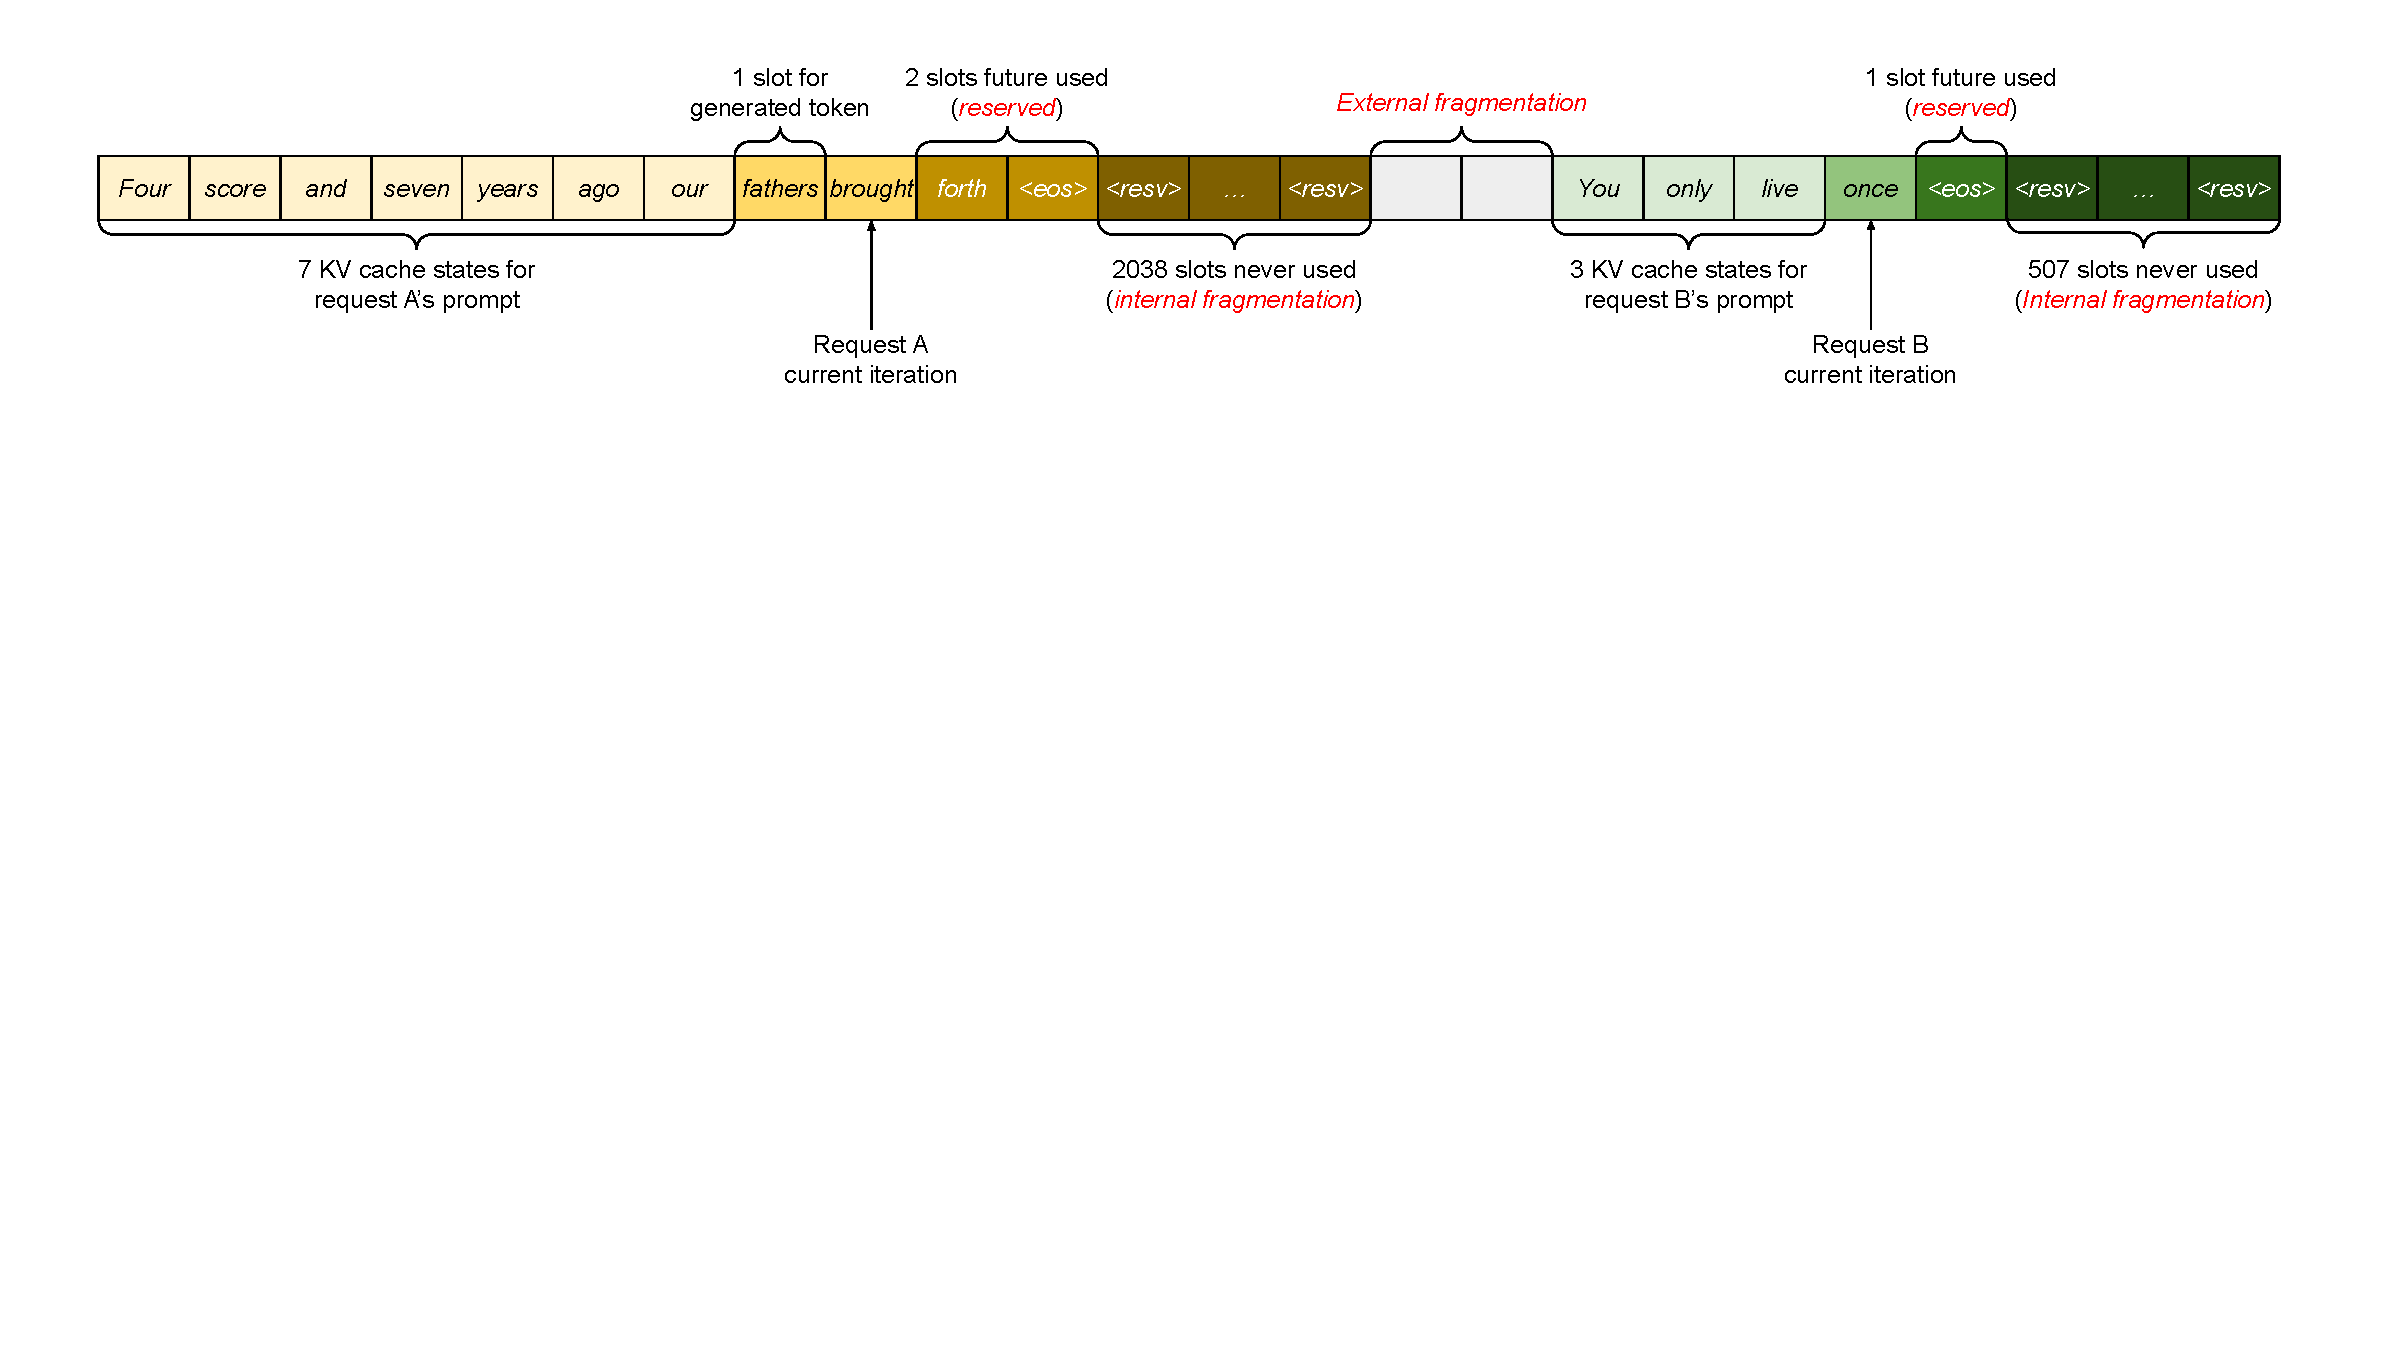
\includegraphics[width=.85\linewidth]{figures/baseline-memory-management.pdf}
    \vspace{-5pt}
    \caption{KV cache memory management in existing systems. Three types of memory wastes -- reserved, internal fragmentation, and external fragmentation -- exist that prevent other requests from fitting into the memory. The token in each memory slot represents its KV cache. Note the same tokens can have different KV cache when at different positions.}
    \label{fig:existing-memory-management}
\end{figure*}

\vspace{-1pt}
\subsection{Batching Techniques for LLMs}
\label{sec:iteration-level-scheduling}

The compute utilization in serving LLMs can be improved by batching multiple requests.
Because the requests share the same model weights, the overhead of moving weights is amortized across the requests in a batch, and can be overwhelmed by the computational overhead when the batch size is sufficiently large.
However, batching the requests to an LLM service is non-trivial for two reasons.
First, the requests may arrive at different times.
A naive batching strategy would either make earlier requests wait for later ones or delay the incoming requests until earlier ones finish, leading to significant queueing delays.
Second, the requests may have vastly different input and output lengths (Fig.~\ref{fig:dataset-length-dist}).
A straightforward batching technique would pad the inputs and outputs of the requests to equalize their lengths, wasting GPU computation and memory.

To address this problem, fine-grained batching mechanisms, such as cellular batching~\cite{gao2018low} and iteration-level scheduling~\cite{yu2022orca}, have been proposed.
Unlike traditional methods that work at the request level, these techniques operate at the iteration level.
After each iteration, completed requests are removed from the batch, and new ones are added.
Therefore, a new request can be processed after waiting for a single iteration, not waiting for the entire batch to complete.
Moreover, with special GPU kernels, these techniques eliminate the need to pad the inputs and outputs.
By reducing the queueing delay and the inefficiencies from padding, the fine-grained batching mechanisms significantly increase the throughput of LLM serving. 

\section{Memory Challenges in LLM Serving}

\label{sec:motivation}

Although fine-grained batching reduces the waste of computing and enables requests to be batched in a more flexible way,
the number of requests that can be batched together is still constrained by GPU memory capacity, particularly the space allocated to store the KV cache. 
In other words, the serving system's throughput is \emph{memory-bound}.
Overcoming this memory-bound requires addressing the following challenges in the memory management:

\heading{Large KV cache.} The KV Cache size grows quickly with the number of requests. As an example, for the 13B parameter OPT model \cite{zhang2022opt}, the KV cache of a single token demands 800 KB of space, calculated as $2$ (key and value vectors) $\times\  5120$ (hidden state size) $\times \  40$ (number of layers) $\times \  2$ (bytes per FP16). Since OPT can generate sequences up to 2048 tokens, the memory required to store the KV cache of one request can be as much as 1.6\,GB. Concurrent GPUs have memory capacities in the tens of GBs. Even if all available memory was allocated to KV cache, only a few tens of requests could be accommodated. Moreover, inefficient memory management can further decrease the batch size, as shown in Fig.~\ref{fig:memory-waste-percentage}. 
Additionally, given the current trends, the GPU's computation speed grows faster than the memory capacity \cite{gholami2021ai}. For example, from NVIDIA A100 to H100, The FLOPS increases by more than 2x, but the GPU memory stays at 80GB maximum. Therefore, we believe the memory will become an increasingly significant bottleneck.


\heading{Complex decoding algorithms.} 
LLM services offer a range of decoding algorithms for users to select from, each with varying implications for memory management complexity. For example, when users request multiple random samples from a single input prompt, a typical use case in program suggestion~\cite{copilot}, the KV cache of the prompt part, which accounts for 12\% of the total KV cache memory in our experiment (\S\ref{sec:eval:beamsearch}), can be shared to minimize memory usage. On the other hand, the KV cache during the autoregressive generation phase should remain unshared due to the different sample results and their dependence on context and position.
The extent of KV cache sharing depends on the specific decoding algorithm employed. In more sophisticated algorithms like beam search~\cite{sutskever2014sequence}, different request beams can share larger portions (up to 55\% memory saving, see \S\ref{sec:eval:beamsearch}) of their KV cache, and the sharing pattern evolves as the decoding process advances. 

\heading{Scheduling for unknown input \& output lengths.} The requests to an LLM service exhibit variability in their input and output lengths. This requires the memory management system to accommodate a wide range of prompt lengths. In addition, as the output length of a request grows at decoding, the memory required for its KV cache also expands and may exhaust available memory for incoming requests or ongoing generation for existing prompts. The system needs to make scheduling decisions, such as deleting or swapping out the KV cache of some requests from GPU memory.

\subsection{Memory Management in Existing Systems}

\label{sec:memory-management-in-existing-systems}

Since most operators in current deep learning frameworks \cite{paszke2019pytorch, olston2017tensorflow} require tensors to be stored in contiguous memory, previous LLM serving systems~\cite{yu2022orca,nvidiaft} also store the KV cache of one request as a contiguous tensor across the different positions. Due to the unpredictable output lengths from the LLM, they statically allocate a chunk of memory for a request based on the request's maximum possible sequence length, irrespective of the actual input or eventual output length of the request. 

Fig.~\ref{fig:existing-memory-management} illustrates two requests: request A with 2048 maximum possible sequence length and request B with a maximum of 512. The chunk pre-allocation scheme in existing systems has three primary sources of memory wastes: \emph{reserved} slots for future tokens, \emph{internal fragmentation} due to over-provisioning for potential maximum sequence lengths, and \emph{external fragmentation} from the memory allocator like the buddy allocator. The external fragmentation will never be used for generated tokens, which is known before serving a request. Internal fragmentation also remains unused, but this is only realized after a request has finished sampling. They are both pure memory waste. 
Although the reserved memory is eventually used, reserving this space for the entire request's duration, especially when the reserved space is large, occupies the space that could otherwise be used to process other requests. We visualize the average percentage of memory wastes in our experiments in Fig.~\ref{fig:memory-waste-percentage}, revealing that the actual effective memory in previous systems can be as low as 20.4\%.

Although compaction~\cite{wang2022pacman} has been proposed as a potential solution to fragmentation, performing compaction in a performance-sensitive LLM serving system is impractical due to the massive KV cache. Even with compaction, the pre-allocated chunk space for each request prevents memory sharing specific to decoding algorithms in existing memory management systems.

\section{Method}

\begin{figure}
    \centering
    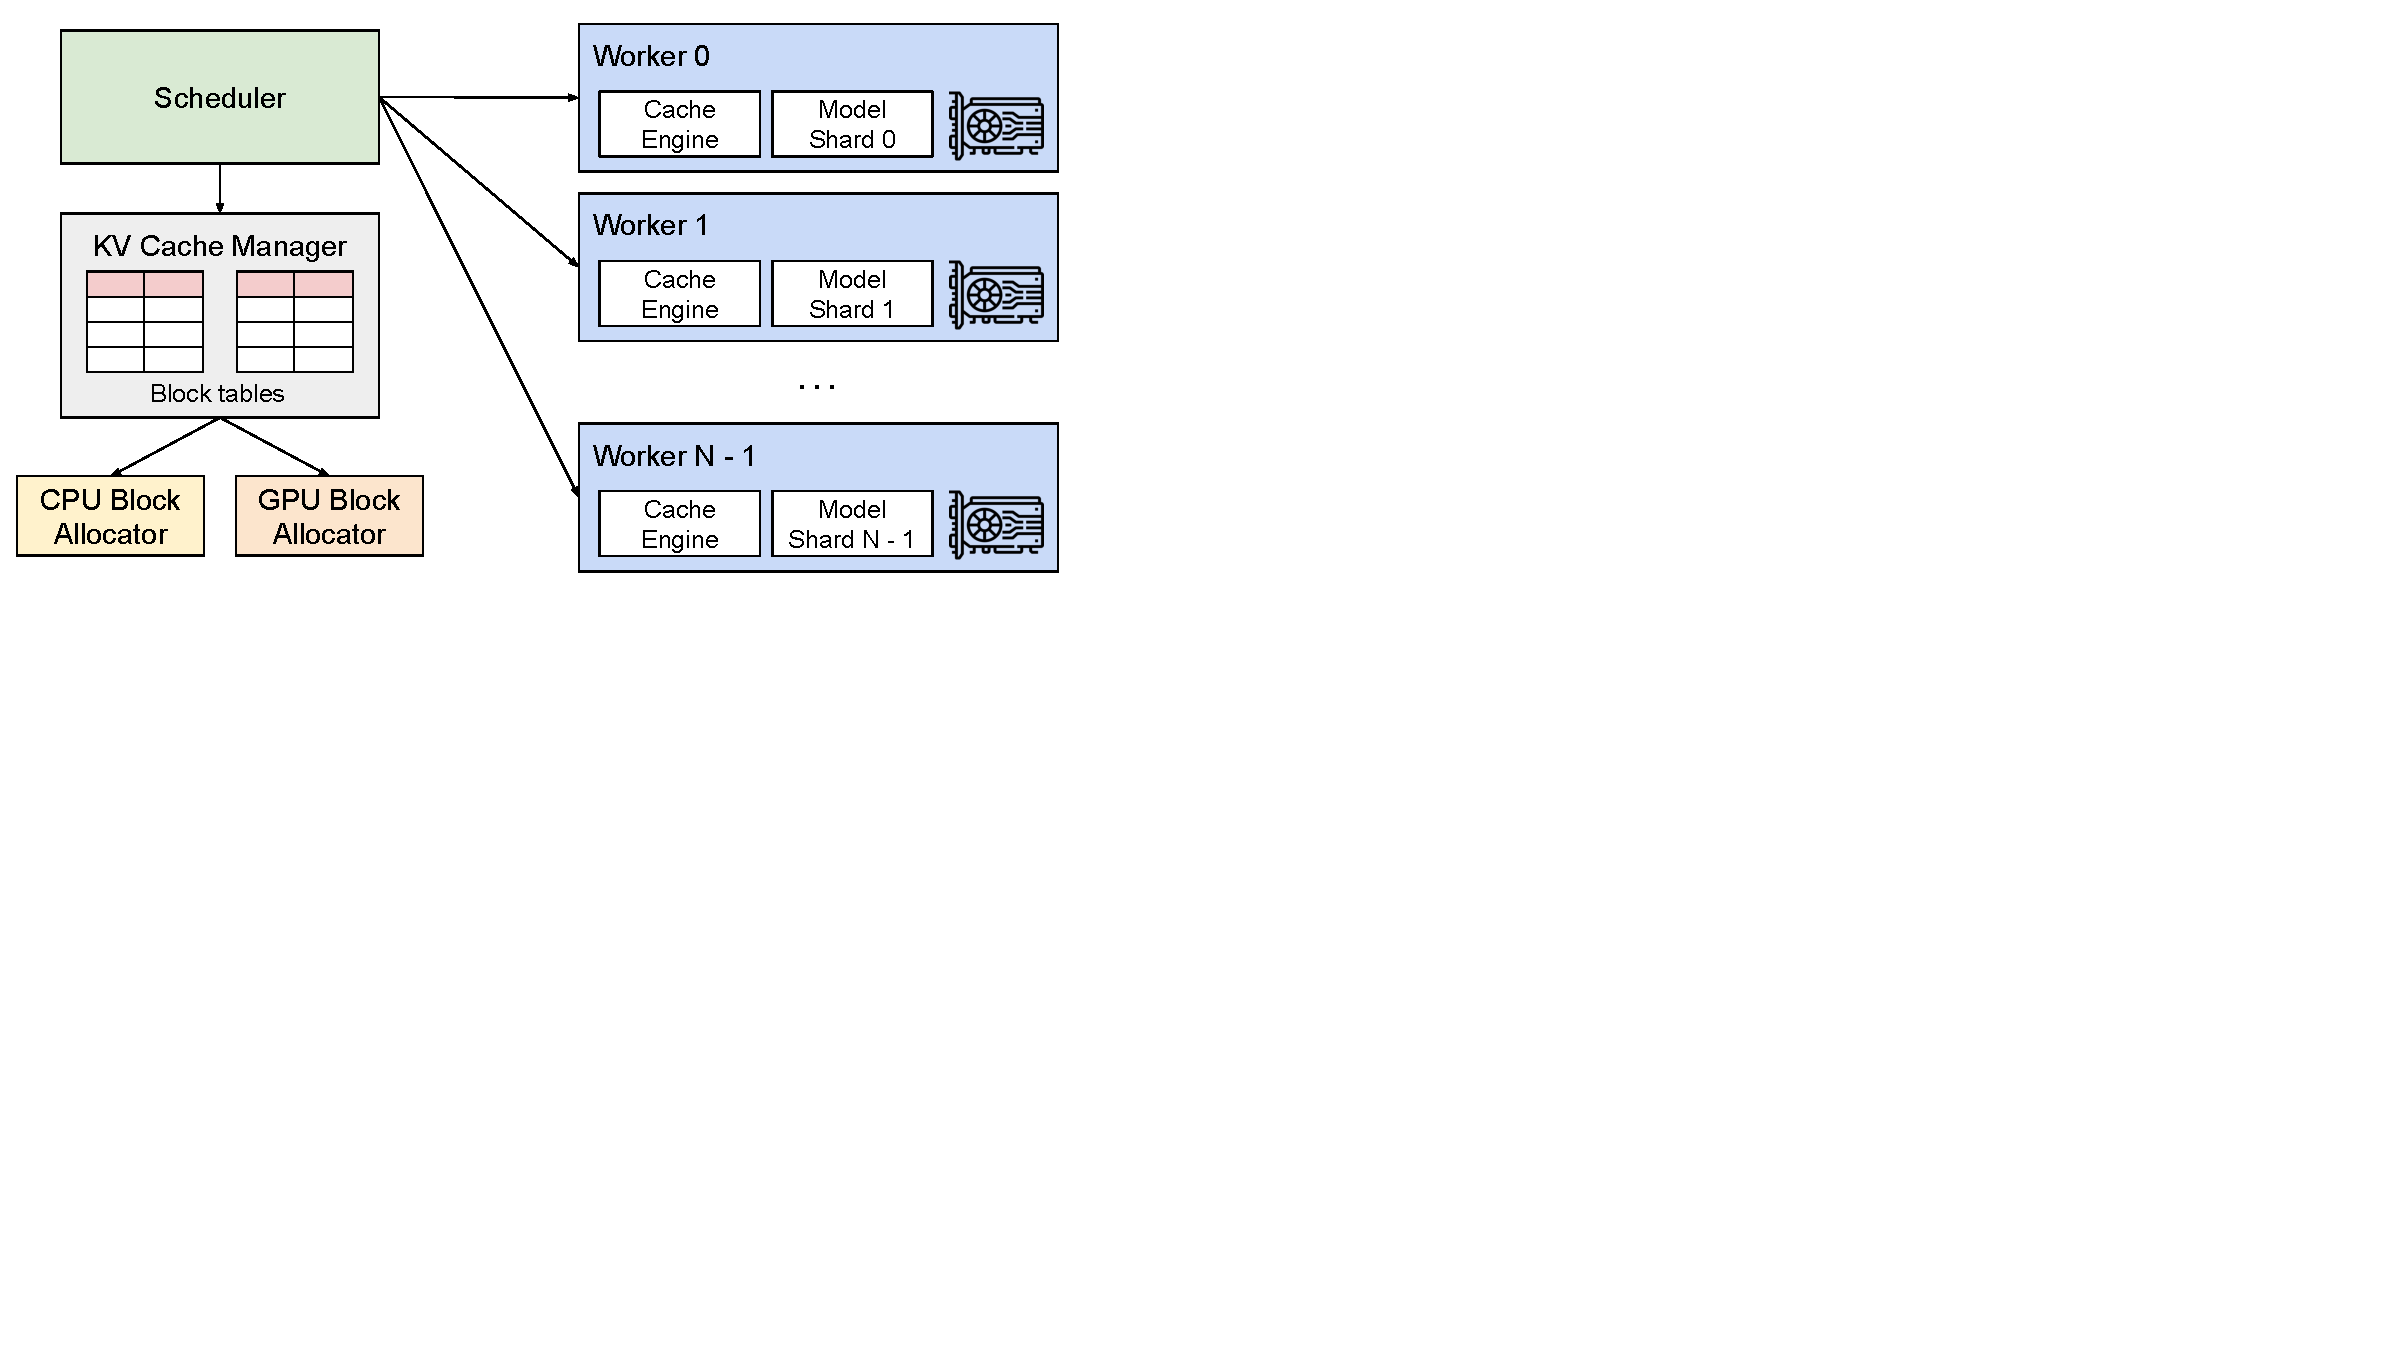
\includegraphics[width=.9\columnwidth]{figures/system-overview.pdf}
    \vspace{-5pt}
    \caption{\sys system overview.} 
    \label{fig:system-overview}
    \vspace{-10pt}
\end{figure}

In this work, we develop a new attention algorithm, \emph{\tech}, and build an LLM serving engine, \emph{\sys}, to tackle the challenges outlined in \S\ref{sec:motivation}. The architecture of \sys is shown in Fig.~\ref{fig:system-overview}. \sys adopts a centralized scheduler to coordinate the execution of distributed GPU workers. The \emph{KV cache manager} effectively manages the KV cache in a paged fashion, enabled by \tech. Specifically, the KV cache manager manages the physical KV cache memory on the GPU workers through the instructions sent by the centralized scheduler.

Next, We describe the \tech algorithm in \S\ref{sec:pagedattention}. With that, we show the design of the KV cache manager in \S\ref{sec:block-space-manager} and how it facilitates \tech in \S\ref{sec:one-sequence-decoding-example}, respectively. Then, we show how this design facilitates effective memory management for various decoding methods (\S\ref{sec:decoding-scenerios}) and handles the variable length input and output sequences (\S\ref{sec:scheduling}). Finally, we show how the system design of \sys works in a distributed setting (\S\ref{sec:distributed}). 

\subsection{\tech}
\label{sec:pagedattention}

To address the memory challenges in \S\ref{sec:motivation}, we introduce \emph{\tech}, an attention algorithm inspired by the classic idea of \emph{paging} \cite{kilburn1962one} in operating systems. Unlike the traditional attention algorithms, \tech allows storing continuous keys and values in non-contiguous memory space. Specifically, \tech partitions the KV cache of each sequence into \emph{KV blocks}. Each block contains the key and value vectors for a fixed number of tokens,\footnote{In Transformer, each token has a set of key and value vectors across layers and attention heads within a layer. All the key and value vectors can be managed together within a single KV block, or the key and value vectors at different heads and layers can each have a separate block and be managed in separate block tables. The two designs have no performance difference and we choose the second one for easy implementation.}  which we denote as \emph{KV block size} ($B$). Denote the key block $K_j = (k_{(j - 1) B + 1}, \ldots, k_{jB})$ and value block $V_j = (v_{(j - 1) B + 1}, \ldots, v_{jB}).$ The attention computation in Eq.~\ref{eq:attention-layer} can be transformed into the following block-wise computation:
\begin{equation}
A_{ij} = \frac{\exp(q_i^\top K_j / \sqrt{d})}{\sum_{t=1}^{\lceil i/B \rceil}\exp(q_i^\top K_t\mathbf{1} / \sqrt{d})}, \ o_i = \sum_{j=1}^{\lceil i/B \rceil} V_j A_{ij}^\top, \label{eq:attention-layer}
\end{equation}
where $A_{ij} = (a_{i,(j - 1) B + 1}, \ldots, a_{i,jB})$ is the row vector of attention score on $j$-th KV block.

During the attention computation, the \tech kernel identifies and fetches different KV blocks separately. We show an example of \tech in Fig.~\ref{fig:pagedattention}: The key and value vectors are spread across three blocks, and the three blocks are not contiguous on the physical memory. At each time, the kernel multiplies the query vector $q_i$ of the query token (``\emph{forth}'') and the key vectors $K_j$ in a block (e.g., key vectors of ``\emph{Four score and seven}'' for block 0) to compute the attention score $A_{ij},$ and later multiplies $A_{ij}$ with the value vectors $V_j$ in a block to derive the final attention output $o_i.$ 

In summary, the \tech algorithm allows the KV blocks to be stored in non-contiguous physical memory, which enables more flexible paged memory management in \sys.

\begin{figure}
    \centering
    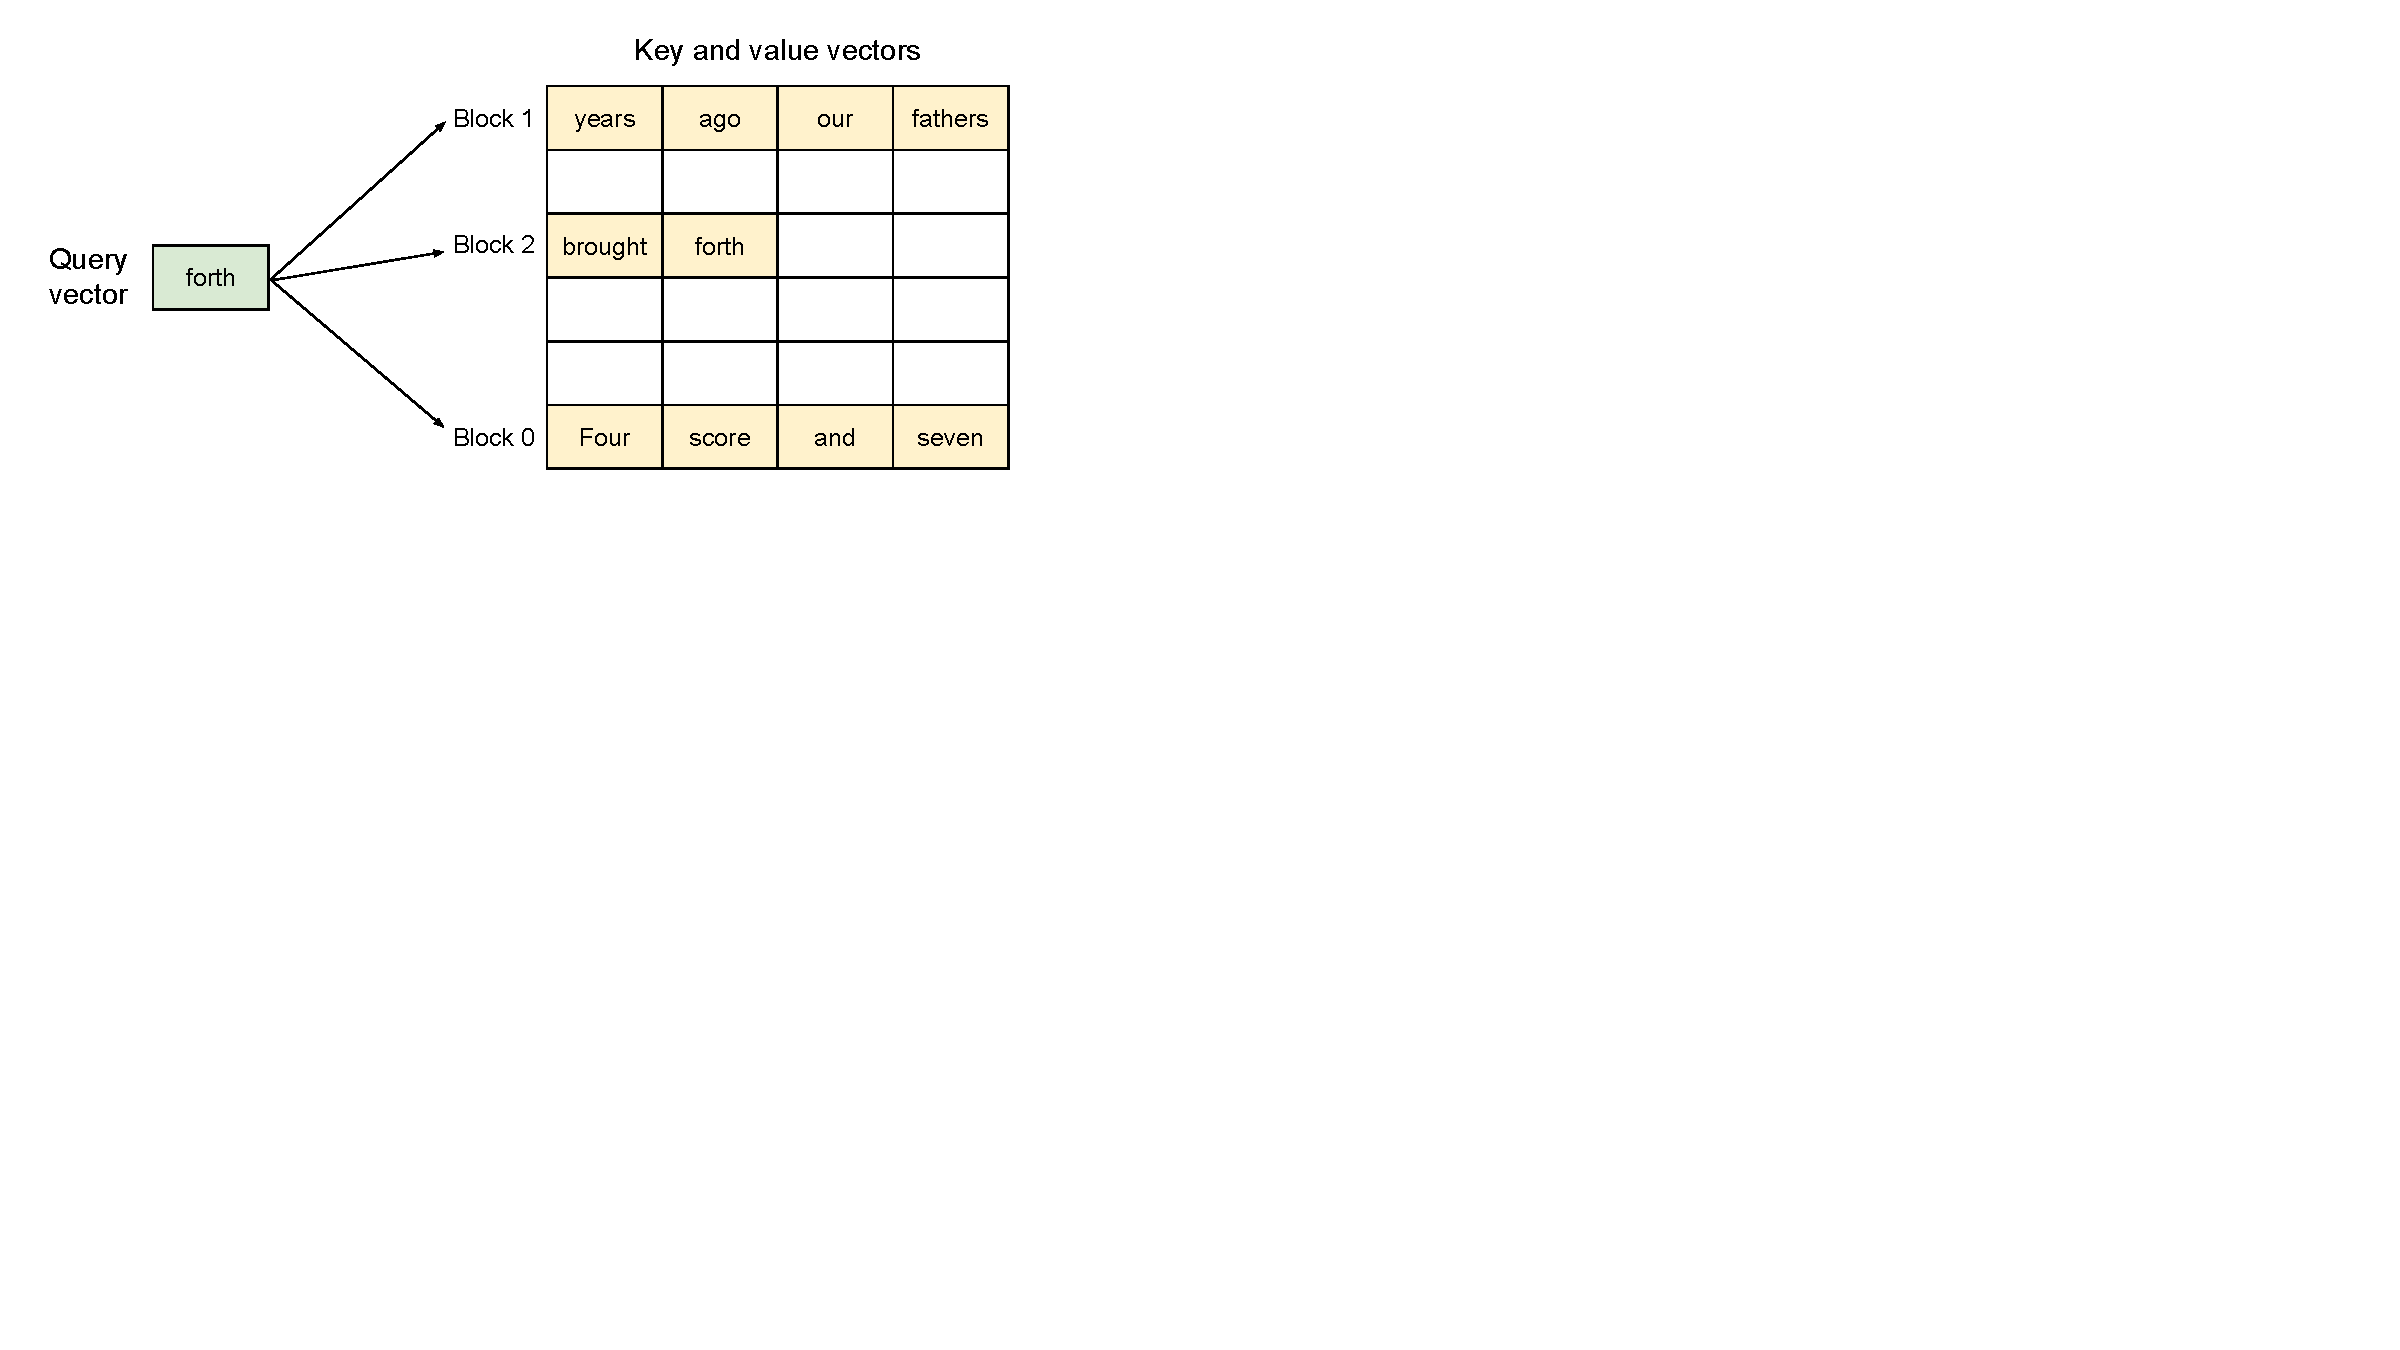
\includegraphics[width=.8\columnwidth]{figures/pagedattention.pdf}
    \vspace{-5pt}
    \caption{Illustration of the \tech algorithm, where the attention key and values vectors are stored as non-contiguous blocks in the memory. }
    \label{fig:pagedattention}
    \vspace{-10pt}
\end{figure}


\subsection{KV Cache Manager}
\label{sec:block-space-manager}

The key idea behind \sys's memory manager is analogous to the \emph{virtual memory} \cite{kilburn1962one} in operating systems. OS partitions memory into fixed-sized \emph{pages} and maps user programs' logical pages to physical pages. Contiguous logical pages can correspond to non-contiguous physical memory pages, allowing user programs to access memory as though it were contiguous. Moreover, physical memory space needs not to be fully reserved in advance, enabling the OS to dynamically allocate physical pages as needed. \sys uses the ideas behind virtual memory to manage the KV cache in an LLM service. Enabled by \tech, we organize the KV cache as fixed-size KV blocks, like pages in virtual memory. 

A request's KV cache is represented as a series of \emph{logical KV blocks}, filled from left to right as new tokens and their KV cache are generated. 
The last KV block's unfilled positions are reserved for future generations.
On GPU workers, a \emph{block engine} allocates a contiguous chunk of GPU DRAM and divides it into \emph{physical KV blocks} (this is also done on CPU RAM for swapping; see \S\ref{sec:scheduling}). The \emph{KV block manager} also maintains \emph{block tables}---the mapping between logical and physical KV blocks of each request. Each block table entry records the corresponding physical blocks of a logical block and the number of filled positions. Separating logical and physical KV blocks allows \sys to dynamically grow the KV cache memory without reserving it for all positions in advance, which eliminates most memory waste in existing systems, as in Fig.~\ref{fig:memory-waste-percentage}. 

\subsection{Decoding with \tech and \sys}
\label{sec:one-sequence-decoding-example}

\begin{figure}
    \centering
    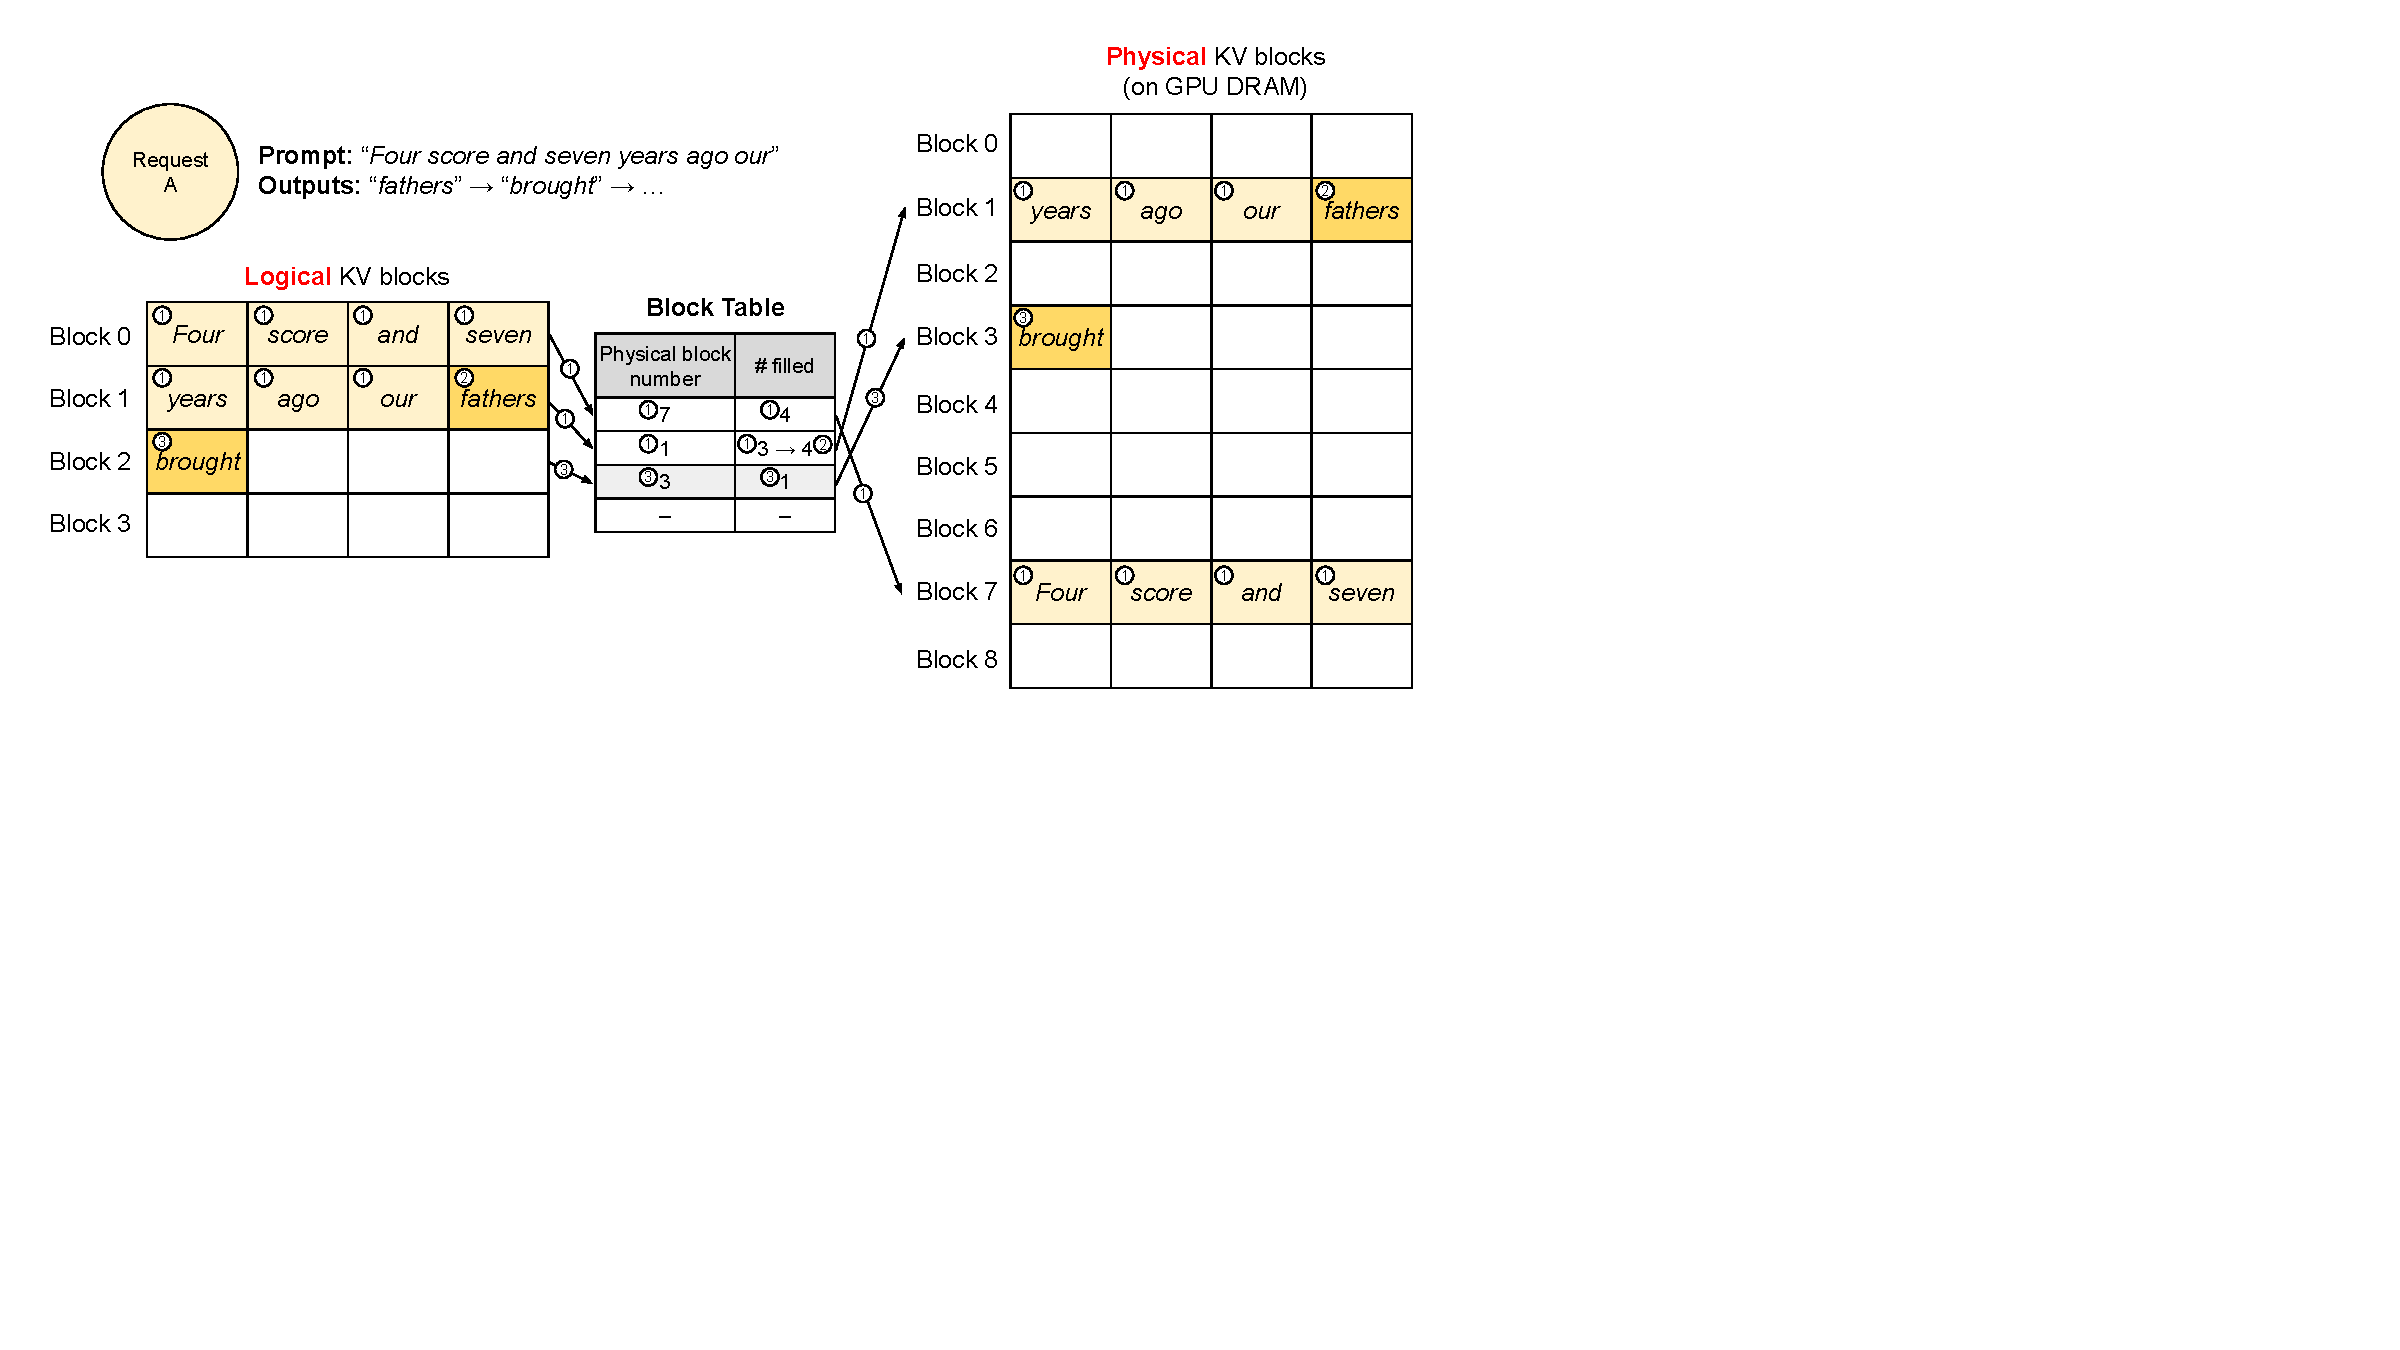
\includegraphics[width=\columnwidth]{figures/logical-and-physical-block-table.pdf}
    \vspace{-15pt}
    \caption{Block table translation in \sys. }
    \label{fig:block-table-translation}
    \vspace{-15pt}
\end{figure}

Next, we walk through an example, as in Fig.~\ref{fig:block-table-translation}, to demonstrate how \sys executes \tech and manages the memory during the decoding process of a single input sequence: \textcircled{\small 1} As in OS's virtual memory, \sys does not require reserving the memory for the maximum possible generated sequence length initially.
Instead, it reserves only the necessary KV blocks to accommodate the KV cache generated during prompt computation. In this case, The prompt has 7 tokens, so \sys maps the first 2 logical KV blocks (0 and 1) to 2 physical KV blocks (7 and 1, respectively). In the prefill step, \sys generates the KV cache of the prompts and the first output token with a conventional self-attention algorithm (e.g., \cite{dao2022flashattention}). \sys then stores the KV cache of the first 4 tokens in logical block 0 and the following 3 tokens in logical block 1. The remaining slot is reserved for the subsequent autoregressive generation phase. 
\textcircled{\small 2} In the first autoregressive decoding step, \sys generates the new token with the \tech algorithm on physical blocks 7 and 1. Since one slot remains available in the last logical block, the newly generated KV cache is stored there, and the block table's \#filled record is updated. \textcircled{\small 3} At the second decoding step, as the last logical block is full, \sys stores the newly generated KV cache in a new logical block; \sys allocates a new physical block (physical block 3) for it and stores this mapping in the block table.

Globally, for each decoding iteration, \sys first selects a set of candidate sequences for batching (more in \S\ref{sec:scheduling}), and allocates the physical blocks for the newly required logical blocks. Then, \sys concatenates all the input tokens of the current iteration (i.e., all tokens for prompt phase requests and the latest tokens for generation phase requests) as one sequence and feeds it into the LLM. During LLM's computation, \sys uses the \tech kernel to access the previous KV cache stored in the form of logical KV blocks and saves the newly generated KV cache into the physical KV blocks. 
Storing multiple tokens within a KV block (block size > 1) enables the \tech kernel to process the KV cache across more positions in parallel, thus increasing the hardware utilization and reducing latency. However, a larger block size also increases memory fragmentation. We study the effect of block size in \S\ref{sec:eval:blocksize}.

Again, \sys dynamically assigns new physical blocks to logical blocks as more tokens and their KV cache are generated. As all the blocks are filled from left to right and a new physical block is only allocated when all previous blocks are full, \sys limits all the memory wastes for a request within one block, so it can effectively utilize all the memory, as shown in Fig.~\ref{fig:memory-waste-percentage}. This allows more requests to fit into memory for batching---hence improving the throughput. Once a request finishes its generation, its KV blocks can be freed to store the KV cache of other requests. 
In Fig.~\ref{fig:multi-sequence-blocks}, we show an example of \sys managing the memory for two sequences. The logical blocks of the two sequences are mapped to different physical blocks within the space reserved by the block engine in GPU workers. The neighboring logical blocks of both sequences do not need to be contiguous in physical GPU memory and the space of physical blocks can be effectively utilized by both sequences.

\begin{figure}
    \centering
    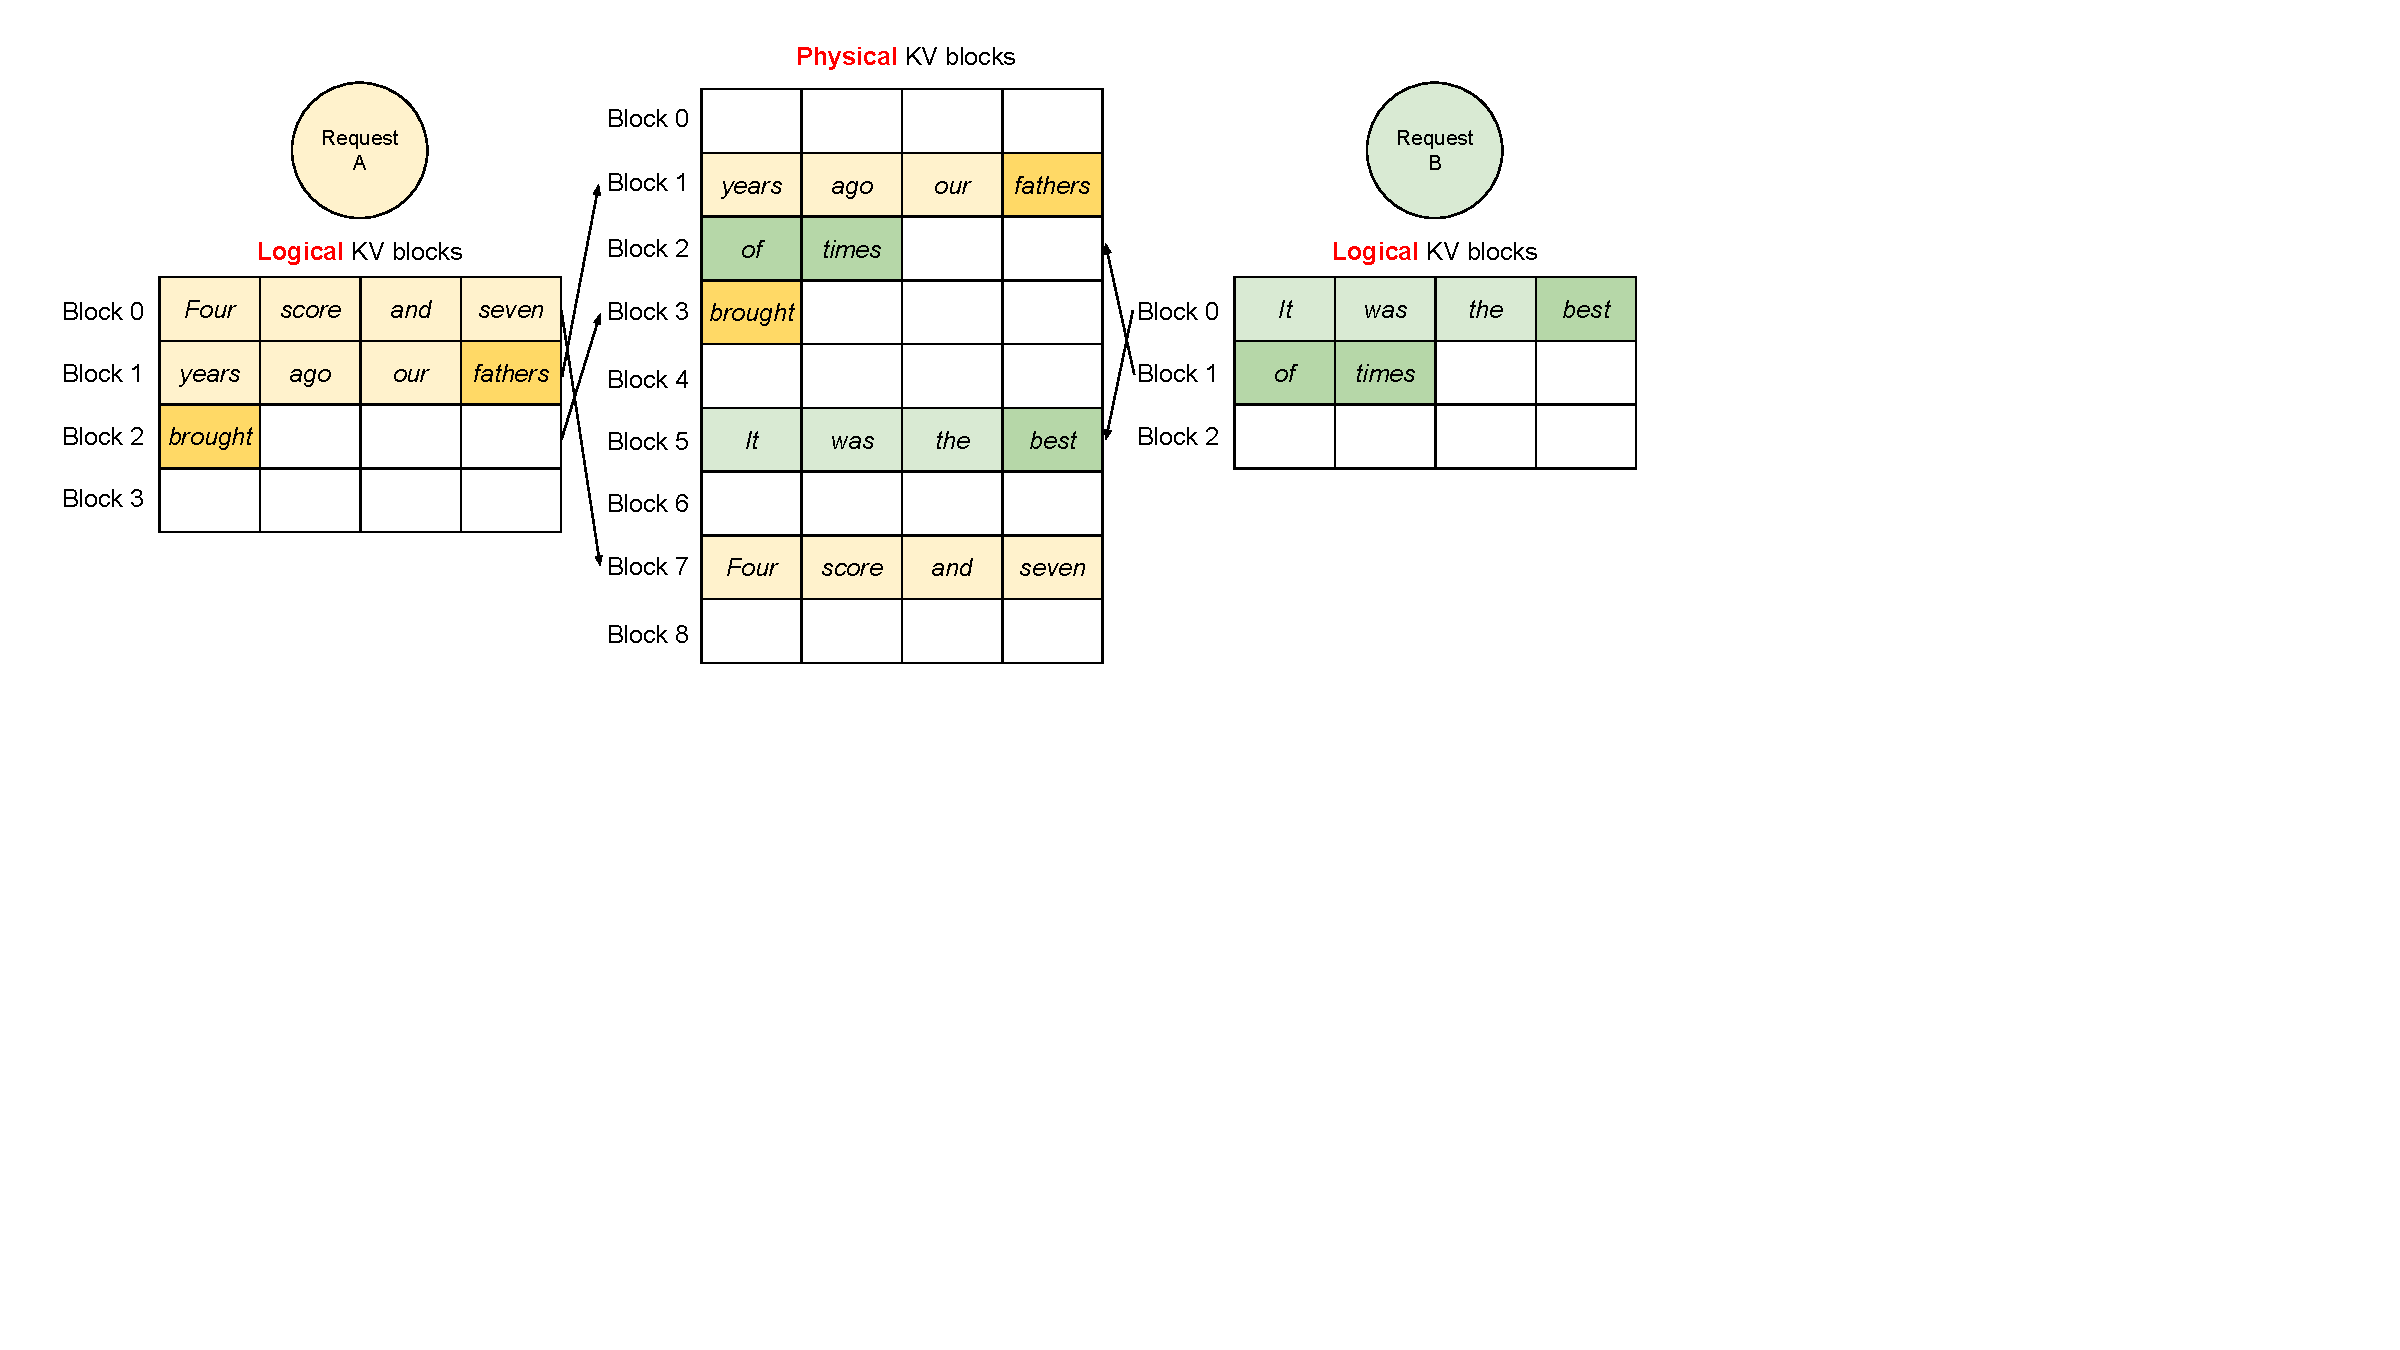
\includegraphics[width=\columnwidth]{figures/multi-sequence-block-mapping.pdf}
    \vspace{-15pt}
    \caption{Storing the KV cache of two requests at the same time in \sys.}
    \label{fig:multi-sequence-blocks}
    \vspace{-10pt}
\end{figure}


\subsection{Application to Other Decoding Scenarios}
\label{sec:decoding-scenerios}

\S\ref{sec:one-sequence-decoding-example} shows how \tech and \sys handle basic decoding algorithms, such as greedy decoding and sampling, that take one user prompt as input and generate a single output sequence. In many successful LLM applications~\cite{copilot, openaiapi}, an LLM service must offer more complex decoding scenarios that exhibit complex accessing patterns and more opportunities for memory sharing. We show the general applicability of \sys on them in this section. 

\heading{Parallel sampling.} 
In LLM-based program assistants~\cite{chen2021evaluating, copilot}, an LLM generates multiple sampled outputs for a single input prompt; users can choose a favorite output from various candidates. 
So far we have implicitly assumed that a request generates a single sequence. In the remainder of this paper, we assume the more general case in which a request generates multiple sequences.
In parallel sampling, one request includes multiple samples sharing the same input prompt, allowing the KV cache of the prompt to be shared as well. Via its \tech and paged memory management, \sys can realize this sharing easily and save memory. 

Fig.~\ref{fig:parallel-decoding} shows an example of parallel decoding for two outputs. 
Since both outputs share the same prompt, we only reserve space for one copy of the prompt's state at the prompt phase; the logical blocks for the prompts of both sequences are mapped to the same physical blocks: the logical block 0 and 1 of both sequences are mapped to physical blocks 7 and 1, respectively. 
Since a single physical block can be mapped to multiple logical blocks, we introduce a \emph{reference count} for each physical block. In this case, the reference counts for physical blocks 7 and 1 are both 2. At the generation phase, the two outputs sample different output tokens and need separate storage for KV cache. 
\sys implements a \emph{copy-on-write} mechanism at the block granularity for the physical blocks that need modification by multiple sequences, similar to the copy-on-write technique in OS virtual memory (e.g., when forking a process).
Specifically, in Fig.~\ref{fig:parallel-decoding}, when sample A1 needs to write to its last logical block (logical block 1), \sys recognizes that the reference count of the corresponding physical block (physical block 1) is greater than 1; it allocates a new physical block (physical block 3), instructs the block engine to copy the information from physical block 1, and decreases the reference count to 1. Next, when sample A2 writes to physical block 1, the reference count is already reduced to 1; thus A2 directly writes its newly generated KV cache to physical block 1. 

In summary, \sys enables the sharing of most of the space used to store the prompts' KV cache across multiple output samples, with the exception of the final logical block, which is managed by a copy-on-write mechanism. By sharing physical blocks across multiple samples, memory usage can be greatly reduced, especially for \emph{long input prompts}. 

\begin{figure}
    \centering
    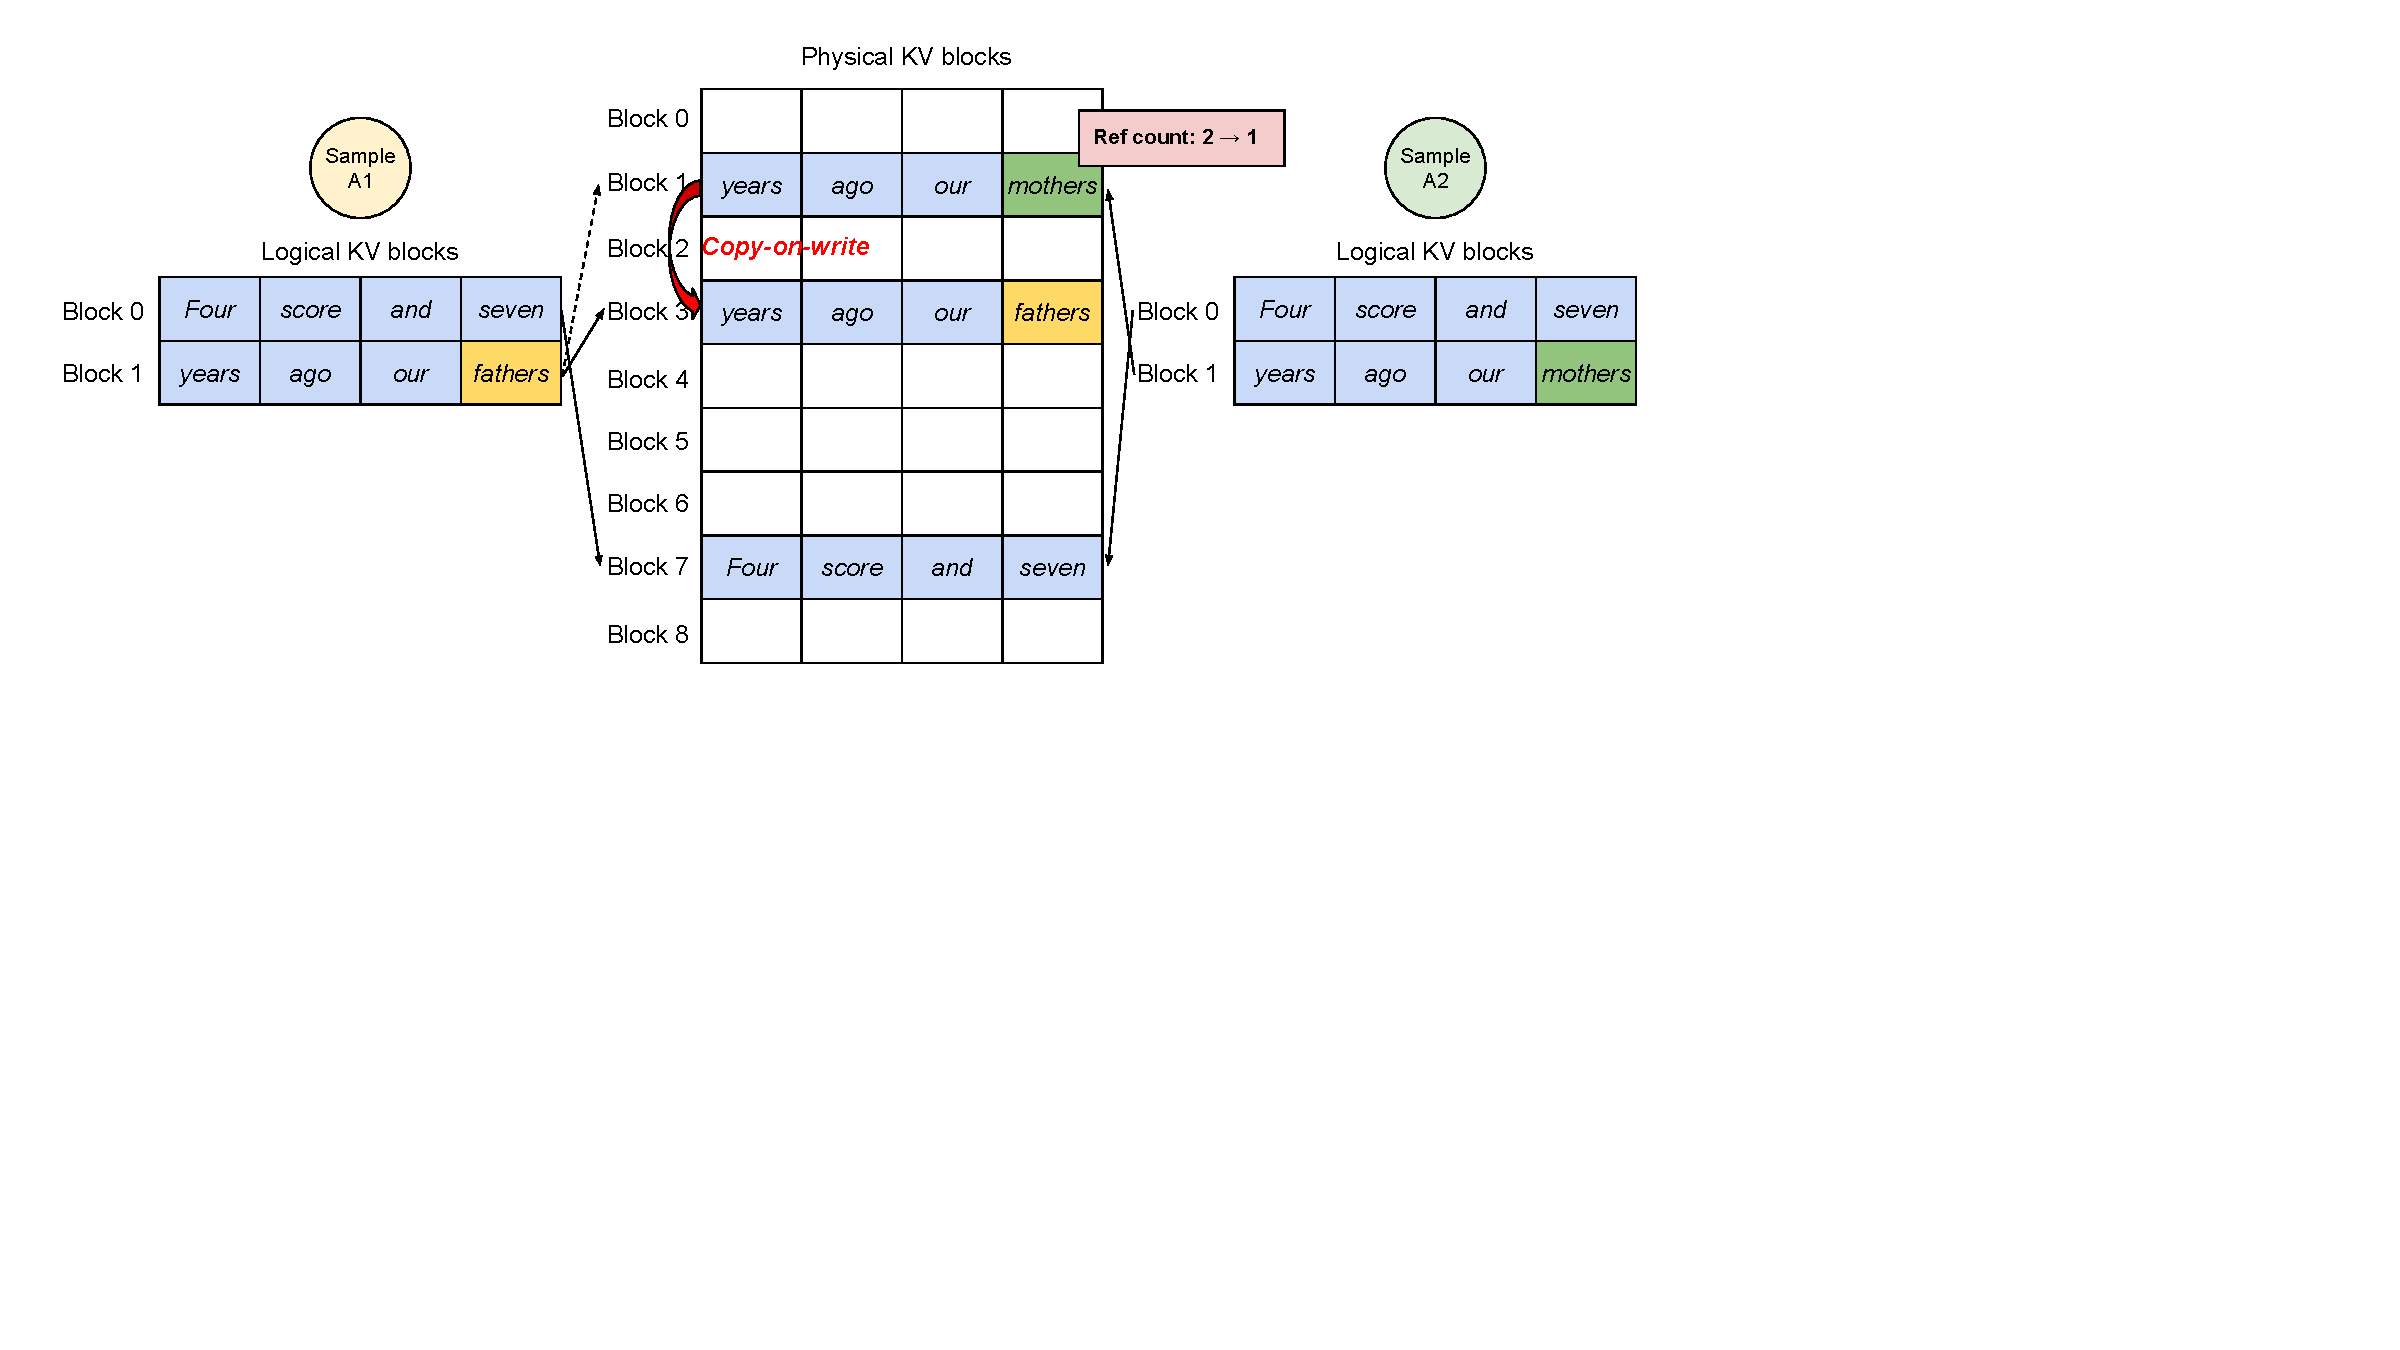
\includegraphics[width=\columnwidth]{figures/parallel-decoding.pdf}
    \vspace{-15pt}
    \caption{Parallel sampling example.}
    \label{fig:parallel-decoding}
    \vspace{-15pt}
\end{figure}

\heading{Beam search.} In LLM tasks like machine translation~\cite{wu2016google}, the users expect the top-$k$ most appropriate translations output by the LLM. Beam search \cite{sutskever2014sequence} is widely used to decode the most probable output sequence from an LLM, as it mitigates the computational complexity of fully traversing the sample space.
The algorithm relies on the \emph{beam width} parameter $k$, which determines the number of top candidates retained at every step. During decoding, beam search expands each candidate sequence in the beam by considering all possible tokens, computes their respective probabilities using the LLM, and retains the top-$k$ most probable sequences out of $k \cdot |V|$ candidates, where $|V|$ is the vocabulary size.

\begin{figure}
    \centering
    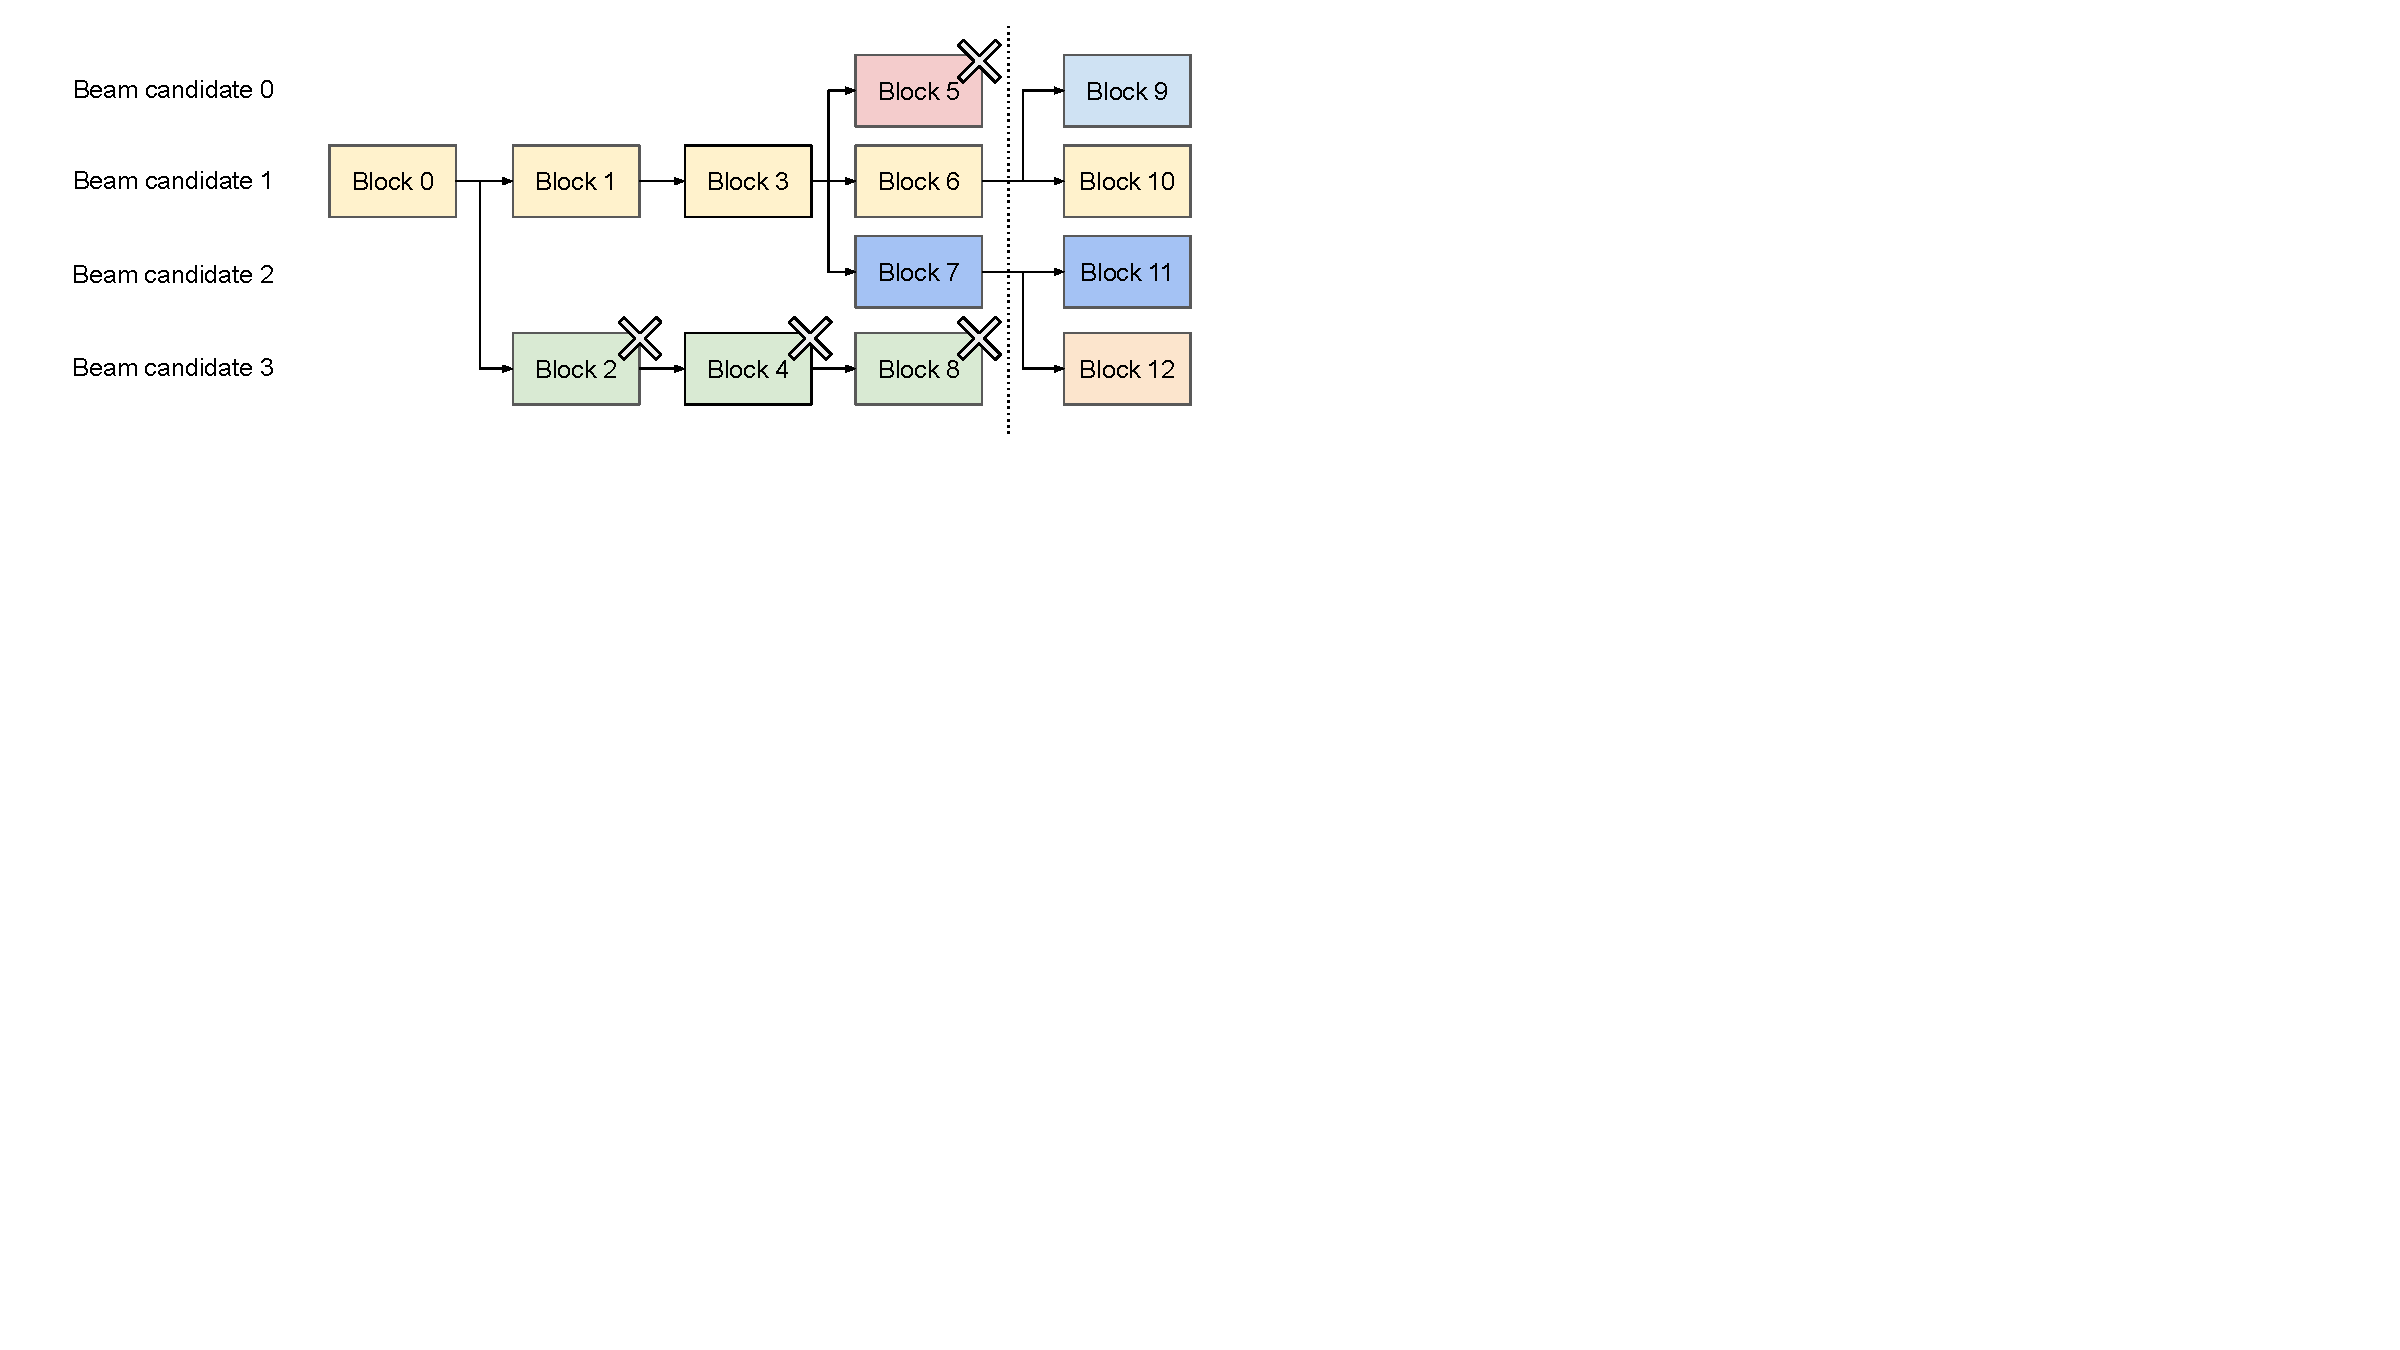
\includegraphics[width=0.9\columnwidth]{figures/beam-search.pdf}
    \vspace{-10pt}
    \caption{Beam search example.}
    \label{fig:beam-search}
    \vspace{-10pt}
\end{figure}

Unlike parallel decoding, beam search facilities sharing not only the initial prompt blocks but also other blocks across different candidates, and the sharing patterns dynamically change as the decoding process advances, similar to the process tree in the OS created by compound forks. 
Fig.~\ref{fig:beam-search} shows how \sys manages the KV blocks for a beam search example with $k = 4$. Prior to the iteration illustrated as the dotted line, each candidate sequence has used 4 full logical blocks. All beam candidates share the first block 0 (i.e., prompt). Candidate 3 digresses from others from the second block. Candidates 0-2 share the first 3 blocks and diverge at the fourth block. At subsequent iterations, the top-4 probable candidates all originate from candidates 1 and 2. As the original candidates 0 and 3 are no longer among the top candidates, their logical blocks are freed, and the reference counts of corresponding physical blocks are reduced. \sys frees all physical blocks whose reference counts reach 0 (blocks 2, 4, 5, 8). Then, \sys allocates new physical blocks (blocks 9-12) to store the new KV cache from the new candidates. Now, all candidates share blocks 0, 1, 3; candidates 0 and 1 share block 6, and candidates 2 and 3 further share block 7.

Previous LLM serving systems require frequent memory copies of the KV cache across the beam candidates. For example, in the case shown in Fig.~\ref{fig:beam-search}, after the dotted line, candidate 3 would need to copy a large portion of candidate 2's KV cache to continue generation. This frequent memory copy overhead is significantly reduced by \sys's physical block sharing. In \sys, most blocks of different beam candidates can be shared. The copy-on-write mechanism is applied only when the newly generated tokens are within an old shared block, as in parallel decoding.  This involves only copying one block of data.

\heading{Shared prefix.} 
Commonly, the LLM user provides a (long) description of the task including instructions and example inputs and outputs, also known as \emph{system prompt} \cite{chatgptuserprompt}.
The description is concatenated with the actual task input to form the prompt of the request. The LLM generates outputs based on the full prompt. Fig.~\ref{fig:share-prompt} shows an example. Moreover, the shared prefix can be further tuned, via prompt engineering, to improve the accuracy of the downstream tasks \cite{li2021prefix, lester2021power}.

For this type of application, many user prompts share a prefix, thus the LLM service provider can store the KV cache of the prefix in advance to reduce the redundant computation spent on the prefix. In \sys, this can be conveniently achieved by reserving a set of physical blocks for a set of predefined shared prefixes by the LLM service provider, as how OS handles shared library across processes. A user input prompt with the shared prefix can simply map its logical blocks to the cached physical blocks (with the last block marked copy-on-write). The prompt phase computation only needs to execute on the user's task input.

\begin{figure}
    \centering
    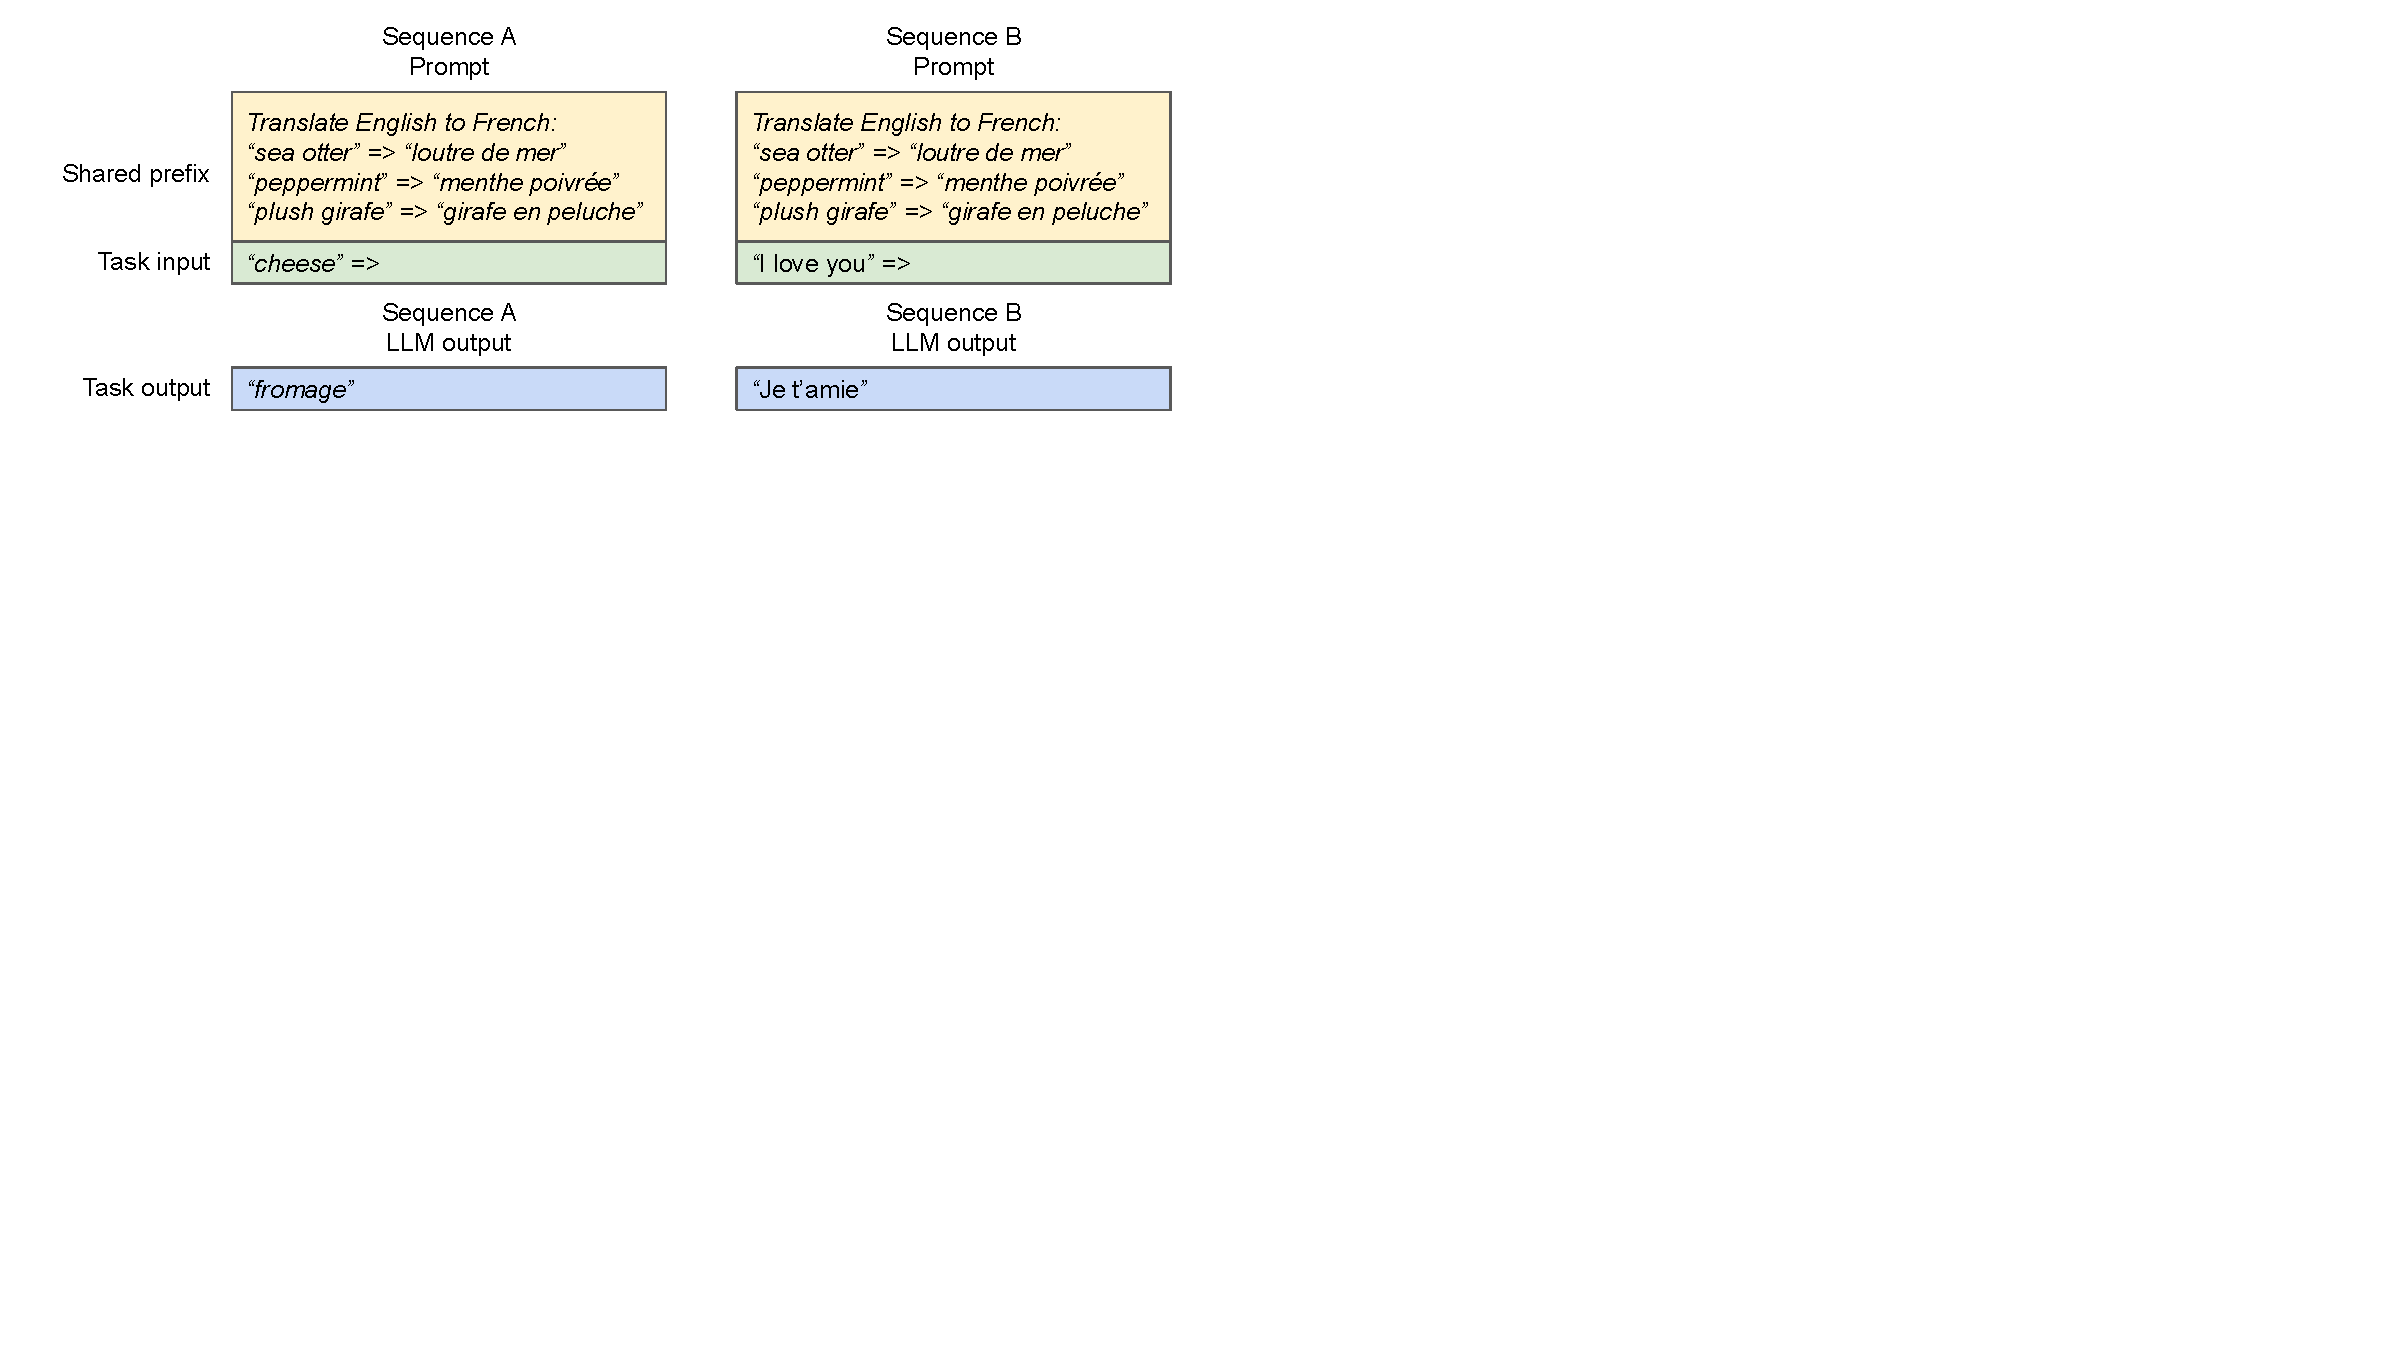
\includegraphics[width=.9\columnwidth]{figures/share-prompt.pdf}
    \vspace{-5pt}
    \caption{Shared prompt example for machine translation. The examples are adopted from~\cite{brown2020language}.}
    \label{fig:share-prompt}
    \vspace{-15pt}
\end{figure}


\heading{Mixed decoding methods.} 
The decoding methods discussed earlier exhibit diverse memory sharing and accessing patterns. Nonetheless, \sys facilitates the simultaneous processing of requests with different decoding preferences, which existing systems \emph{cannot} efficiently do.
This is because \sys conceals the complex memory sharing between different sequences via a common mapping layer that translates logical blocks to physical blocks. The LLM and its execution kernel only see a list of physical block IDs for each sequence and do not need to handle sharing patterns across sequences. Compared to existing systems, this approach broadens the batching opportunities for requests with different sampling requirements, ultimately increasing the system's overall throughput.

\subsection{Scheduling and Preemption}
\label{sec:scheduling}

When the request traffic surpasses the system’s capacity, \sys must prioritize a subset of requests. In \sys, we adopt the first-come-first-serve (FCFS) scheduling
policy for all requests, ensuring fairness and preventing starvation. When \sys needs to preempt requests, it ensures
that the earliest arrived requests are served first and the
latest requests are preempted first.

LLM services face a unique challenge: the input prompts for an LLM can vary significantly in length, and the resulting output lengths are not known a priori, contingent on both the input prompt and the model. As the number of requests and their outputs grow, \sys can run out of the GPU's physical blocks to store the newly generated KV cache. There are two classic questions that \sys needs to answer in this context: (1) Which blocks should it evict? (2) How to recover evicted blocks if needed again? Typically, eviction policies use heuristics to predict which block will be accessed furthest in the future and evict that block. Since in our case we know that all blocks of a sequence are accessed together, we implement an all-or-nothing eviction policy, i.e., either evict all or none of the blocks of a sequence. Furthermore, multiple sequences within one request (e.g., beam candidates in one beam search request) are gang-scheduled as a \emph{sequence group}. The sequences within one sequence group are always preempted or rescheduled together due to potential memory sharing across those sequences. 
To answer the second question of how to recover an evicted block, we consider two techniques:

\heading{Swapping.} This is the classic technique used by most virtual memory implementations which copy the evicted pages to a swap space on the disk. In our case, we copy evicted blocks to the CPU memory. As shown in Fig.~\ref{fig:system-overview}, besides the GPU block allocator, \sys includes a CPU block allocator to manage the physical blocks swapped to CPU RAM. When \sys exhausts free physical blocks for new tokens, it selects a set of sequences to evict and transfer their KV cache to the CPU. Once it preempts a sequence and evicts its blocks, \sys stops accepting new requests until all preempted sequences are completed. Once a request completes, its blocks are freed from memory, and the blocks of a preempted sequence are brought back in to continue the processing of that sequence.
Note that with this design, the number of blocks swapped to the CPU RAM never exceeds the number of total physical blocks in the GPU RAM, so the swap space on the CPU RAM is bounded by the GPU memory allocated for the KV cache. 

\heading{Recomputation.} In this case, we simply recompute the KV cache when the preempted sequences are rescheduled. Note that recomputation latency can be significantly lower than the original latency, as the tokens generated at decoding can be concatenated with the original user prompt as a new prompt---their KV cache at all positions can be generated in one prompt phase iteration.

The performances of swapping and recomputation depend on the bandwidth between CPU RAM and GPU memory and the computation power of the GPU. We examine the speeds of swapping and recomputation in \S\ref{sec:eval:scheduling}.

\subsection{Distributed Execution}
\label{sec:distributed}
Many LLMs have parameter sizes exceeding the capacity of a single GPU~\cite{brown2020language, chowdhery2022palm}. Therefore, it is necessary to partition them across distributed GPUs and execute them in a model parallel fashion~\cite{zheng2022alpa, li2023alpaserve}. This calls for a memory manager capable of handling distributed memory. \sys is effective in distributed settings by supporting the widely used Megatron-LM style tensor model parallelism strategy on Transformers~\cite{shoeybi2019megatron}. 
This strategy adheres to an SPMD (Single Program Multiple Data) execution schedule, wherein the linear layers are partitioned to perform block-wise matrix multiplication, and the the GPUs constantly synchronize intermediate results via an all-reduce operation. Specifically, the attention operator is split on the attention head dimension, each SPMD process takes care of a subset of attention heads in multi-head attention.

We observe that even with model parallel execution, each model shard still processes the same set of input tokens, thus requiring the KV Cache for the same positions. Therefore, \sys features a single KV cache manager within the centralized scheduler, as in Fig.~\ref{fig:system-overview}. Different GPU workers share the manager, as well as the mapping from logical blocks to physical blocks. 
This common mapping allows GPU workers to execute the model with the physical blocks provided by the scheduler for each input request.
Although each GPU worker has the same physical block IDs, a worker only stores a portion of the KV cache for its corresponding attention heads.

In each step, the scheduler first prepares the message with input token IDs for each request in the batch, as well as the block table for each request. Next, the scheduler broadcasts this control message to the GPU workers. Then, the GPU workers start to execute the model with the input token IDs. In the attention layers, the GPU workers read the KV cache according to the block table in the control message. During execution, the GPU workers synchronize the intermediate results with the all-reduce communication primitive without the coordination of the scheduler, as in \cite{shoeybi2019megatron}. In the end, the GPU workers send the sampled tokens of this iteration back to the scheduler. In summary, GPU workers do not need to synchronize on memory management as they only need to receive all the memory management information at the beginning of each decoding iteration along with the step inputs.

\section{Implementation}
\label{sec:impl}

\begin{table}[tp]\centering\small
\caption{Model sizes and server configurations.}
\vspace{-10pt}
\scalebox{0.9}{
\begin{tabular}{@{} l c c c @{}} \toprule
Model size & \textbf{13B} & \textbf{66B} & \textbf{175B} \\
\midrule
GPUs & A100 & 4$\times$A100 & 8$\times$A100-80GB \\
Total GPU memory & 40 GB & 160 GB & 640 GB \\
Parameter size & 26 GB & 132 GB & 346 GB \\
\midrule
Memory for KV cache & 12 GB & 21 GB & 264 GB \\
Max. \# KV cache slots & 15.7K & 9.7K & 60.1K \\
\bottomrule
\end{tabular}
}
\vspace{-5pt}
\label{table:model_config}
\end{table}


\sys is an end-to-end serving system with a FastAPI~\cite{fastapi} frontend and a GPU-based inference engine.
The frontend extends the OpenAI API~\cite{openaiapi} interface, allowing users to customize sampling parameters for each request, such as the maximum sequence length and the beam width $k$.
The \sys engine is written in 8.5K lines of Python and 2K lines of C++/CUDA code.
We develop control-related components including the scheduler and the block manager in Python while developing custom CUDA kernels for key operations such as \tech.
For the model executor, we implement popular LLMs such as GPT~\cite{brown2020language}, OPT~\cite{zhang2022opt}, and LLaMA~\cite{touvron2023llama} using PyTorch~\cite{paszke2019pytorch} and Transformers~\cite{wolf2020transformers}.
We use NCCL~\cite{nccl} for tensor communication across the distributed GPU workers.

\subsection{Kernel-level Optimization}
\label{sec:impl-kernel}

Since \tech introduces memory access patterns that are not efficiently supported by existing systems, we develop several GPU kernels for optimizing it.
(1) \emph{Fused reshape and block write.}
In every Transformer layer, the new KV cache are split into blocks, reshaped to a memory layout optimized for block read, then saved at positions specified by the block table. To minimize kernel launch overheads, we fuse them into a single kernel.
(2) \emph{Fusing block read and attention.}
We adapt the attention kernel in FasterTransformer~\cite{nvidiaft} to read KV cache according to the block table and perform attention operations on the fly.
To ensure coalesced memory access, we assign a GPU warp to read each block.
Moreover, we add support for variable sequence lengths within a request batch.
(3) \emph{Fused block copy.}
Block copy operations, issued by the copy-on-write mechanism, may operate on discontinuous blocks.
This can lead to numerous invocations of small data movements if we use the \texttt{cudaMemcpyAsync} API.
To mitigate the overhead, we implement a kernel that batches the copy operations for different blocks into a single kernel launch.

\begin{figure}[t]
     \centering
     \begin{subfigure}[b]{0.5\linewidth}
         \centering
         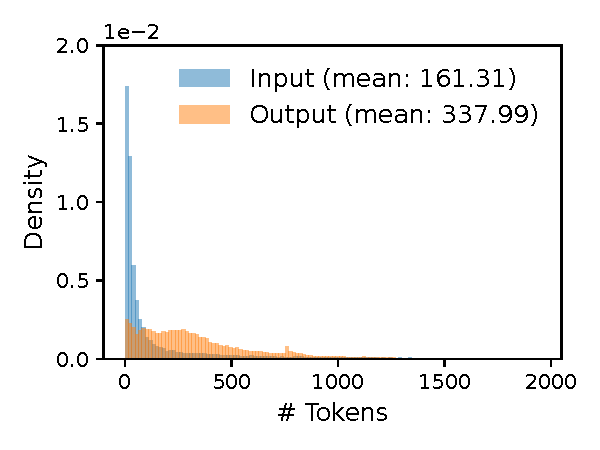
\includegraphics[width=1\columnwidth]{figures/experiments/sharegpt_hist.pdf}
         \vskip -0.1in
         \caption{\small ShareGPT}
     \end{subfigure}%\hfill
     \begin{subfigure}[b]{0.5\linewidth}
         \centering
         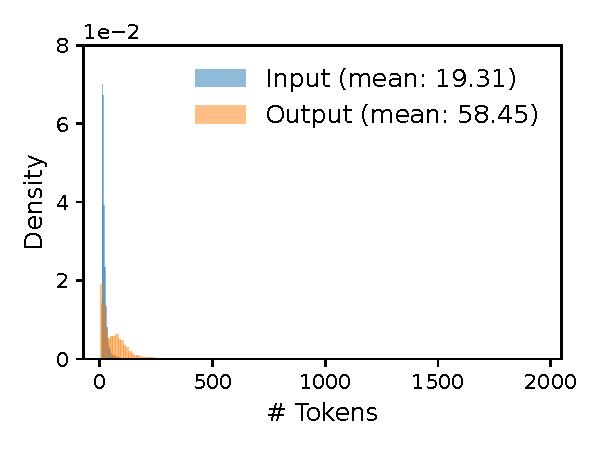
\includegraphics[width=1\columnwidth]{figures/experiments/alpaca_hist.pdf}
         \vskip -0.1in
         \caption{\small Alpaca}
     \end{subfigure}%\hfill
     \vskip -0.1in
     \caption{Input and output length distributions of the (a) ShareGPT and (b) Alpaca datasets.}     
     \vspace{-10pt}
\label{fig:dataset-length-dist}
\end{figure}

\subsection{Supporting Various Decoding Algorithms}

\sys implements various decoding algorithms using three key methods: \texttt{fork}, \texttt{append}, and \texttt{free}.
The \texttt{fork} method creates a new sequence from an existing one.
The \texttt{append} method appends a new token to the sequence.
Finally, the \texttt{free} method deletes the sequence.
For instance, in parallel sampling, \sys creates multiple output sequences from the single input sequence using the \texttt{fork} method.
It then adds new tokens to these sequences in every iteration with \texttt{append}, and deletes sequences that meet a stopping condition using \texttt{free}.
The same strategy is also applied in beam search and prefix sharing by \sys.
We believe future decoding algorithms can also be supported by combining these methods.

\section{Evaluation}
\label{sec:eval-cloak}

In this section, we evaluate \system's efficacy in protecting artists from
style mimicry. We first describe the datasets, models, and experimental
configurations used in our tests. Then we present the results of \system's
protection in a variety of settings. Due to \system's highly visual nature,
we evaluate its performance using both direct visual assessment by
\textbf{human artists} in a user study, and \textbf{automated metrics} (see
\S\ref{sec:metrics} for details).

\para{Summary of results.} Over $93\%$ of artists surveyed believe \system{}
effectively protects artists' styles from AI style mimicry
attacks. Protection efficacy remains high in challenging settings, like when
the mimic has access to unprotected artwork. \system{} also achieves high
protection performance against a real-world mimicry-as-a-service platform. Of
our $1156$ artist participants, over $92\%$ found the perturbations
introduced by cloaking small enough not to disrupt the value of their art,
and over $88\%$ would like to use \system{} to protect their own artwork from
mimicry attacks.

\secspace
\subsection{Experiment Setup}
\label{sec:cloak-setup}

\para{Mimicry dataset. } We evaluate \system's performance in protecting the styles of the following two groups of artists: 

\vspace{-0.2cm}
\begin{packed_itemize}
\item {\em Current artists}: $4$ professional artists let us use their
  artwork in our experiments. These artists have different styles and
  backgrounds (\eg full-time/freelancers, watercolor painters/digital
  artists, well-known/independent). Each provided us with between $26$ to
  $34$ \textit{private} original art pieces for our experiments. We use
  perceptual hashing~\cite{ke2004efficient} to verify that none of these are
  included in existing public datasets used to train generic text-to-image
  models (e.g.~\cite{schuhmann2022laion,changpinyo2021conceptual}).  

\item {\em Historical artists}: We also evaluate \system{}'s protection on
  $195$ historical artists (\eg van Gogh, Monet) from the WikiArt
  dataset~\cite{saleh2015large}. The WikiArt dataset contains 42,129 art
  pieces from $195$ artists. Each art piece is labeled with its genre (\eg
  impressionism, cubism). We randomly sampled $30$ art pieces from each
  artist to use in style mimicry attacks. Generic text-to-image models found
  online have been trained on some artwork from these artists. Using this art
  simulates a more challenging scenario in which a famous artist attempts
  to disrupt a model that already understands their style.
\end{packed_itemize}
\vspace{-0.2cm}

\para{Mimicry attack setup. } We recreate the strongest-possible mimicry
attack scenario, based on techniques used in real-world mimicry
incidents~\cite{ruiz2022dreambooth,sam-steal,hollie-steal},
that works as follows. First, we take art pieces from the victim artist $V$
and generate a text caption for each piece using an image captioning
model~\cite{luo2022vc}. \revise{The pretrained image captioning model generates a short 
sentence to describe the image. We found that this model can correctly caption protected images (examples in Figure~\ref{fig:data-examples}), likely because \system{} focuses on perturbing style features while the captioning models focus on image content.} Then, we append the artist's name to each caption,
\eg ``mountain range \textit{by Vincent van Gogh}''. Finally, we fine-tune a pre-trained generic text-to-image model
(details below) on the caption/image pairs. 

We use $80\%$ of the art pieces from the victim artists to fine-tune models
that mimic each artist's style, reserving the rest for testing. We fine-tune
for $3000$ optimization steps, which we find achieves the best mimicry
performance (Figure~\ref{fig:success-iter} in Appendix). We then use the
fine-tuned, style-specific model to generate mimicked artwork in style of
each victim artist. We query the model using the generated captions (which
include $V$'s name) from the held-out test artwork set. We generate $5$
pieces of mimicked art for each text caption using different random seeds and
compare these to the real victim art pieces with this caption. Additional
details on training and generation parameters, as well as its sensitivity to
random seed selection and the number of training art pieces are in Appendix~\ref{app:mimicry}.  

% Fine-tuning a style-specific mimicry model takes 56.4 minutes on average on one Titan RTX GPU~\footnote{This takes longer than real-world mimicry incidents because we finetune more steps for better mimicry performance.}. 

\para{Text-to-image models.} We use two state-of-the-art, public, generic text-to-image models in our experiments: 

\vspace{-0.2cm}
\begin{packed_itemize}
\item \textit{Stable Diffusion (SD)}: Stable Diffusion is a popular and
  high-performing open-source text-to-image model~\cite{stable2-1},trained
  on 11.5 million images from the LAION dataset~\cite{schuhmann2022laion}. SD
  training takes over 277 GPU months (on A100 GPU) and costs around
  \$600K~\cite{stable2-1}. SD uses diffusion methods to generate images and
  achieves state-of-the-art performance on several
  benchmarks~\cite{rombach2022high}. Viewed as one of the best open-source
  models, SD has powered many recent developments in text-to-image
  generation~\cite{blender-plugin,novelai-update,gimp,aigame}. We
  use SD version 2.1 in the paper~\cite{stable2-1}, the most up-to-date
  version as of December 2022.  

\item \textit{DALL$\cdot$E-mega (\dalleM)}: \dalleM-mega, an updated version
  of the more well-known \dalleM-mini, is an open-source model based on
  OpenAI's \dalleM~1~\cite{ramesh2021zero}. The model leverages a VAE for
  image generation and is trained on 17 million images from three different
  datasets~\cite{sharma-etal-2018-conceptual,changpinyo2021conceptual,thomee2016yfcc100m}. Training
  takes 2 months on 256 TPUs~\cite{mini-training}. While \dalleM~ performs
  worse than diffusion-based models like SD, we use it to evaluate how
  \system~generalizes to different model architectures.  
\end{packed_itemize}

\vspace{-0.2cm}

\para{\system~configuration. } We generate cloaks for each of victim $V$'s
art pieces following the methodology of \S\ref{sec:design-details}. First, we
use the target selection algorithm to select a target style $T$. We choose
from a set of $1119$ candidate target styles, collected by querying the
WikiArt dataset with artist and genre names, \eg ``Impressionism painting by
Monet''~\footnote{One artist may paint in multiple styles, resulting in
  multiple candidate target styles from a single artist.}. We then style
transfer each victim art piece into the target style leveraging the style
transfer functionality of stable diffusion model (stable diffusion model has
both text-to-image and style transfer functionality). \revise{A style transfer model takes
in an original image and a target prompt as input. Leveraging a similar diffusion process, the model
modifies the original image to a style similar to that described in the target prompt. More information on style transfer can be found in ~\cite{saharia2022palette}}. Finally, we optimize a cloak for each art piece
using Eq.~\ref{eq:optdetail} by running the Adam optimizer for $500$
steps. \revise{We benchmark \system{}'s runtime on artwork with resolution ranging 
from $512$ to $6000$ pixels, using SD's feature extractor (ViT model with 83 million parameters). } It takes an average of $1.2$ mins on Titan RTX GPU and $7.3$ mins on a
single Intel i7 CPU to generate a cloak for a single piece of art. 

In our initial experiments, we assume \system{} generates cloaks using the
same image feature extractor as the mimic (e.g. SD's or \dalleM's feature
extractor). We relax this assumption and evaluate
\system{}'s performance when artists and mimics use different feature
extractors in \S\ref{sec:robust-eval}.

\secspace
\subsection{Evaluation Metrics} 
\label{sec:metrics}

We evaluate our protection performance using both visual assessment and feedback from
human artists, and a scalable metric. Here, we describe the setup of our
evaluation study and define the exact metrics used for evaluation.  

% \vspace{-0.2cm}
% \begin{packed_itemize}
\para{Artist-rated protection success rate (Artist-rated PSR): } The user
studies ask artists to rate the performance of \system. We generate a dataset
of mimicry attacks on $13$ victim artists (the $4$ current artists and $9$
randomly chosen historical artists) across $23$ protection scenarios
(including ones in \S\ref{sec:counter}). For each participant, we randomly
select a set of mimicry attacks out of these $13 \times 23$ settings and ask
them to evaluate protection success.  For each mimicry attempt, we show
participants $4$ mimicked art pieces and $4$ original art pieces from the
victim artist. \revise{Using original art pieces as an indicator of the human
artist's style,} we ask participants to consider the mimicked art, and rate the success of 
\system{}'s
protection on a 5-level Likert scale (ranging from ``not successful at all''
to ``very successful''). Each mimicry attempt is evaluated by at least $10$
participants. We define \textit{artist-rated PSR} as the percent of
participants who rated \system{}'s protection as ``successful'' or ``very
successful.''  Our user studies primarily focus on artists, as they would be
most affected by this technology. We found though, that not all current
artists despise AI art, and some view it as a new avenue for a different form
of artistry.

\para{CLIP-based genre shift: } We define a new metric based on
CLIP~\cite{radford2021learning}, using the intuition that \system{} succeeds
if the mimicked art has been impacted enough by \system{} to be classified
into a \textit{different art genre} from the artist's original artwork. We
leverage CLIP model's ability to classify art images into art genres. Given a
set of mimicked art targeting an artist $V$, we define \textit{CLIP-based
  genre shift rate} as the percentage of mimicked art whose top 3 predicted
genres do not contain $V$'s original genre. A higher genre shift rate means
more mimicked art belongs to a different genre from the victim artist, and thus
means more successful protection.

To calculate the genre shift we use a set of $27$ historical genres from
WikiArt dataset and $13$ digital art genres~\cite{digital-styles} as the
candidate output labels. In Appendix~\ref{app:clip}, we show that a
pre-trained CLIP model is able to achieve high genre classification
performance. We report the average CLIP-based genre shift for all 199 victim
artists across all mimicked artworks.

We use CLIP-based genre shift as a supplemental metric to evaluate \system{}
because it is only able to detect style changes at the granularity of art
genres.
% checks whether the mimicked artwork belongs to a different
% art genre as artist's true genre.
However, mimicry attacks also fail when
\system{} causes the mimicked artwork quality to be very low, something that 
CLIP cannot measure. Measuring the quality of generated image has been a
challenging and ongoing research problem in computer
vision~\cite{kynkaanniemi2022role,blau2018perception,karras2020training}.


\begin{figure*}[t]
  \centering
  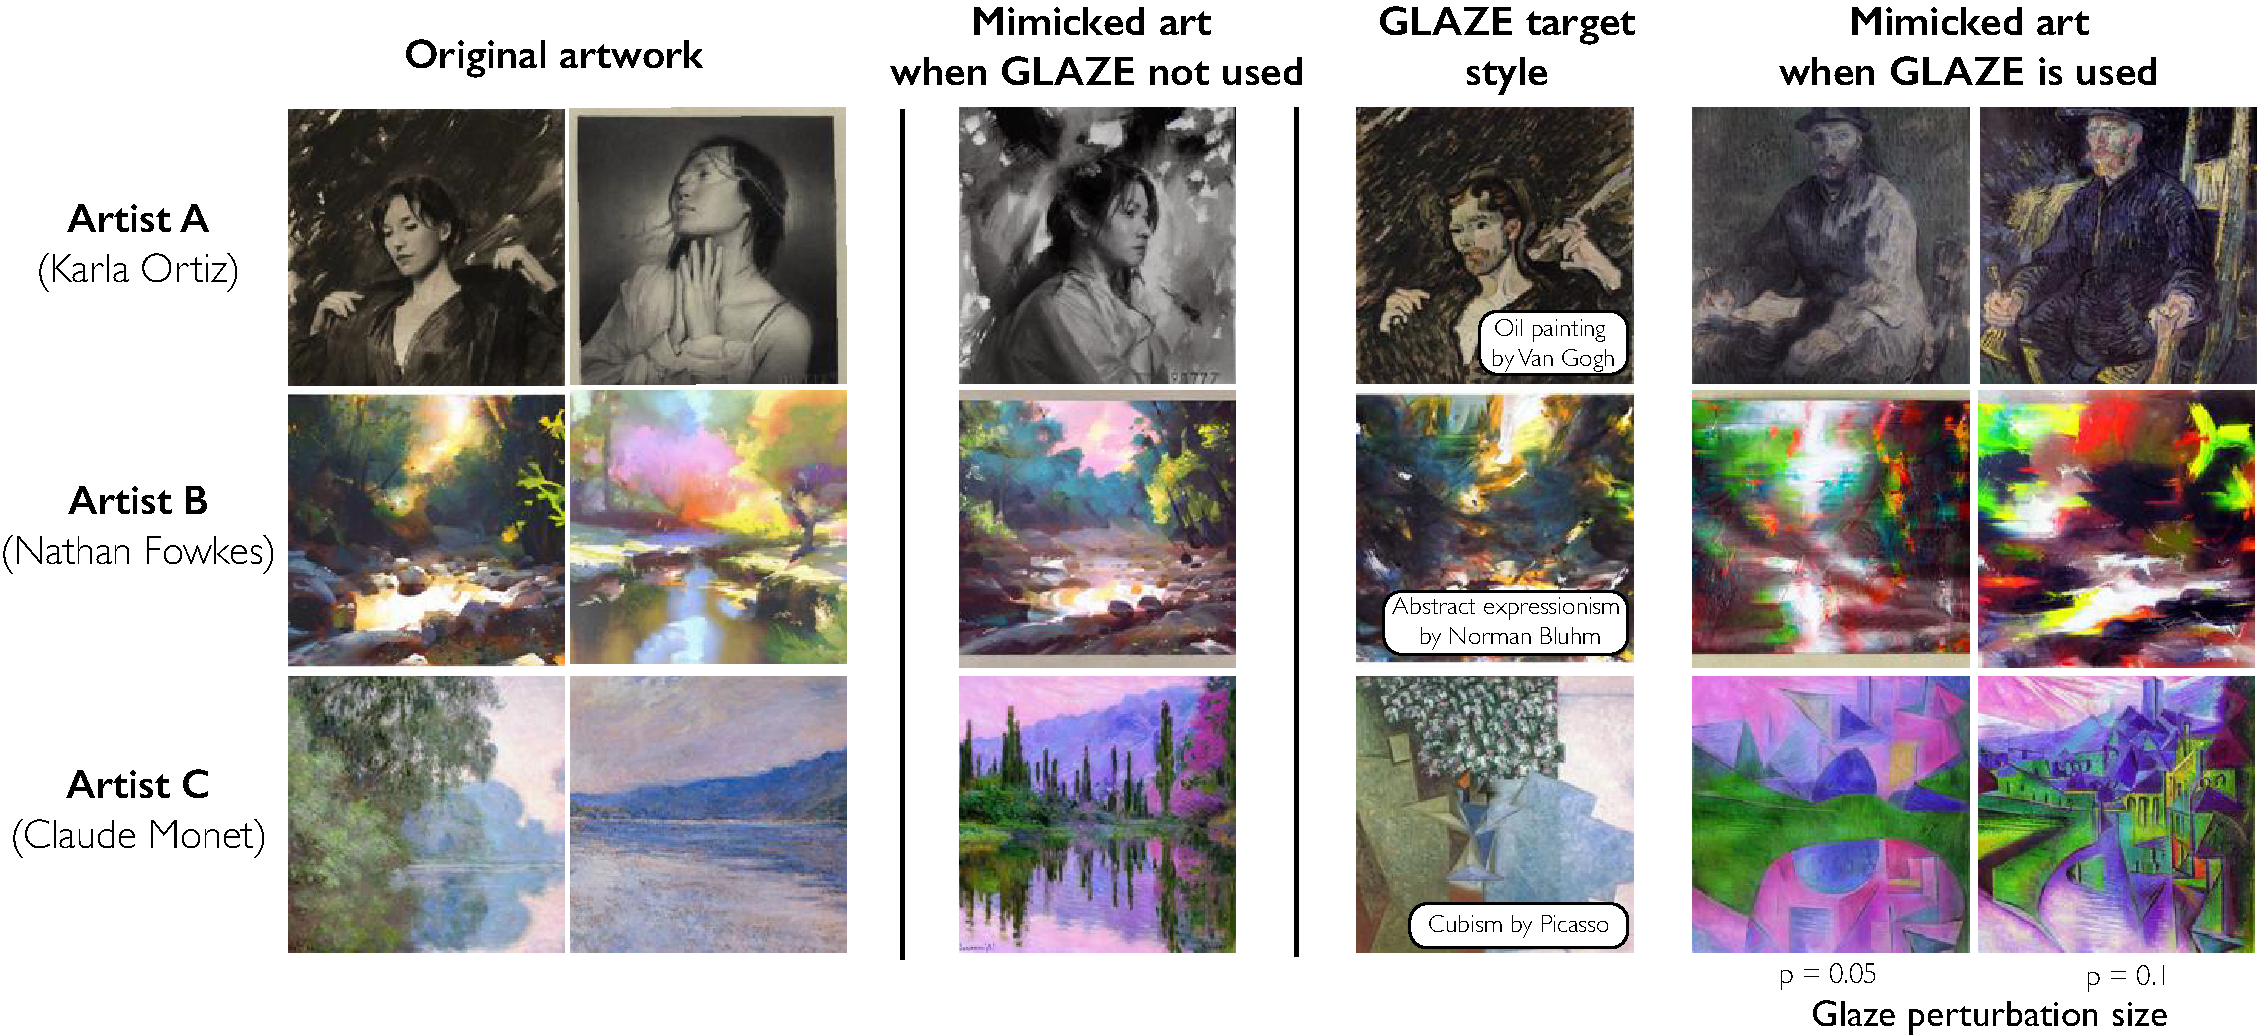
\includegraphics[width=0.9\linewidth]{plots/eval/big-result-full-emily.pdf}
  \vspace{-0.1in}
  \caption{Example \system{} protection results for three artists. {\bf
      Columns 1-2}: artist's original artwork; {\bf column 3}: mimicked
    artwork when artist does not use protection; {\bf column 4}:
    style-transferred artwork (original artwork in column 1 is the source)
    used for cloak optimization and the name of target style; {\bf column
      5-6}: mimicked artwork when artist uses cloaking protection with
    perturbation budget $p=0.05$ or $p=0.1$ respectively. All mimicry
    examples here use SD-based models.
  } %The images can be zoomed for a closer look when viewing the paper digitally. )}
  \label{fig:core-res}
\end{figure*}

\begin{table}[t]
  \centering
  \resizebox{0.5\textwidth}{!}{
  \centering
\begin{tabular}{cccccc}
\toprule
\multirow{2}{*}{\textbf{\begin{tabular}[c]{@{}c@{}} \\ Generic \\ model\end{tabular}}} & \multirow{2}{*}{\textbf{\begin{tabular}[c]{@{}c@{}}\\ Artist \\ dataset\end{tabular}}} & \multicolumn{2}{c}{\textbf{w/o \system{}}} & \multicolumn{2}{c}{\textbf{w/ \system{} (p=0.05)}} \\ \cmidrule{3-6} 
 &  & \begin{tabular}[c]{@{}c@{}}Artist-rated \\ PSR\end{tabular} & \begin{tabular}[c]{@{}c@{}}CLIP-based \\ genre shift\end{tabular} & \begin{tabular}[c]{@{}c@{}}Artist-rated \\ PSR\end{tabular} & \begin{tabular}[c]{@{}c@{}}CLIP-based \\ genre shift\end{tabular} \\ \midrule
\multirow{2}{*}{SD} & Current & $4.6 \pm 0.3\%$ & $2.4 \pm 0.2\%$ & $94.3 \pm 0.8\%$ & $96.4 + 0.5\%$ \\
 & Historical & $4.2 \pm 0.2\%$ & $1.3 \pm 0.2\%$ & $93.3 + 0.6\%$ & $96.0 + 0.3\%$ \\ \midrule
\multirow{2}{*}{\dalleM~} & Current & $31.9 \pm 3.5\%$ & $6.4 \pm 0.8\%$ & $97.4 \pm 0.2\%$ & $97.4 + 0.3\%$ \\
 & Historical & $29.8 \pm 2.4\%$ & $5.8 \pm 0.6\%$ & $96.8 \pm 0.3\%$ & $97.1 + 0.2\%$ \\ \bottomrule
\end{tabular}
  }
  \vspace{-0.1in}
  \caption{\system{} has a high protection success rate, as measured by
    artists and CLIP, against style mimicry attacks. We compare protection
    success when artists do not use \system{} vs. when they do (with
    perturbation budget 0.05). }
  \label{tab:psr-core-table}
  \vspace{-0.3cm}
\end{table}

\begin{figure*}[t]
  \centering
  \begin{minipage}{0.32\textwidth}
  \centering
  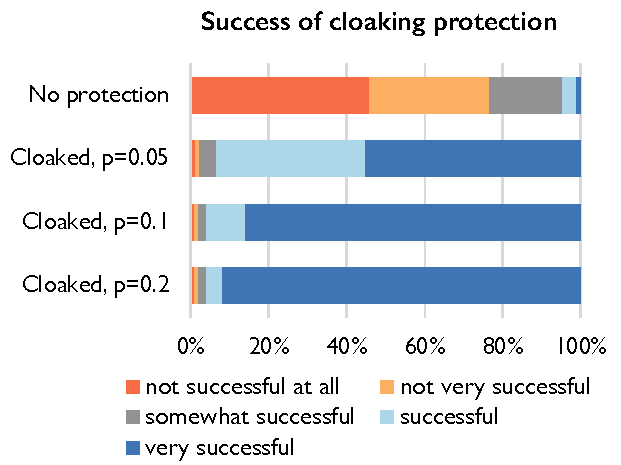
\includegraphics[width=1\columnwidth]{plots/eval/user-cloak-budget.pdf}
  \vspace{-0.23in}
  \caption{\system{}'s cloaking protection success increases as cloak perturbation budget increases. The top row of the figure shows baseline performance with the mimic trains on uncloaked images (p=0). }
  \label{fig:budget-increase}
  \end{minipage}
  \hfill
    \centering
    \begin{minipage}{0.32\textwidth}
  \vspace{0.23in}
  \centering
    \resizebox{1\textwidth}{!}{
    \begin{tabular}{lcc}
    \toprule
    \multicolumn{1}{c}{\textbf{\begin{tabular}[c]{@{}c@{}}Perturbation\\ budget\end{tabular}}} & \textbf{\begin{tabular}[c]{@{}c@{}}Artist-rated \\ PSR\end{tabular}} & \textbf{\begin{tabular}[c]{@{}c@{}}CLIP-based \\ genre shift\end{tabular}} \\ \midrule
    0 (no cloak) & $4.6 \pm 1.4\%$ & $2.4 \pm 0.8\%$ \\
    0.05 & $93.3 \pm 0.6\%$ & $96.0 \pm 0.3\%$ \\
    0.1 & $95.9 \pm 0.4\%$& $98.2 \pm 0.1\%$ \\
    0.2 & $96.1 \pm 0.3\%$ & $98.5 \pm 0.1\%$ \\ \bottomrule
    \end{tabular}
    }
    \vspace{0.13in}
    \captionof{table}{Performance of our system (artist-rated protection success rate and CLIP-based genre shift rate) increases as the perturbation budget increases. (SD model, averaged over all victim artists). }
    \label{tab:budget-increase-sd}
  \end{minipage}
  \hfill
\centering
  \begin{minipage}{0.32\textwidth}
  \centering
  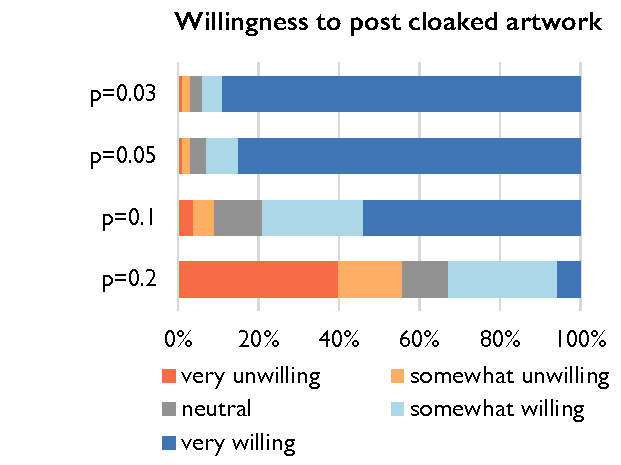
\includegraphics[width=1\columnwidth]{plots/eval/user-accept.pdf}
  \vspace{-0.23in}
  \caption{Artists' willingness to post cloaked artwork in place of the original decreases as perturbation budget of the cloaks increases. }
  \label{fig:artist-accept} 
  \end{minipage}
    \hfill
\end{figure*}

\begin{figure}[t]
  \centering
  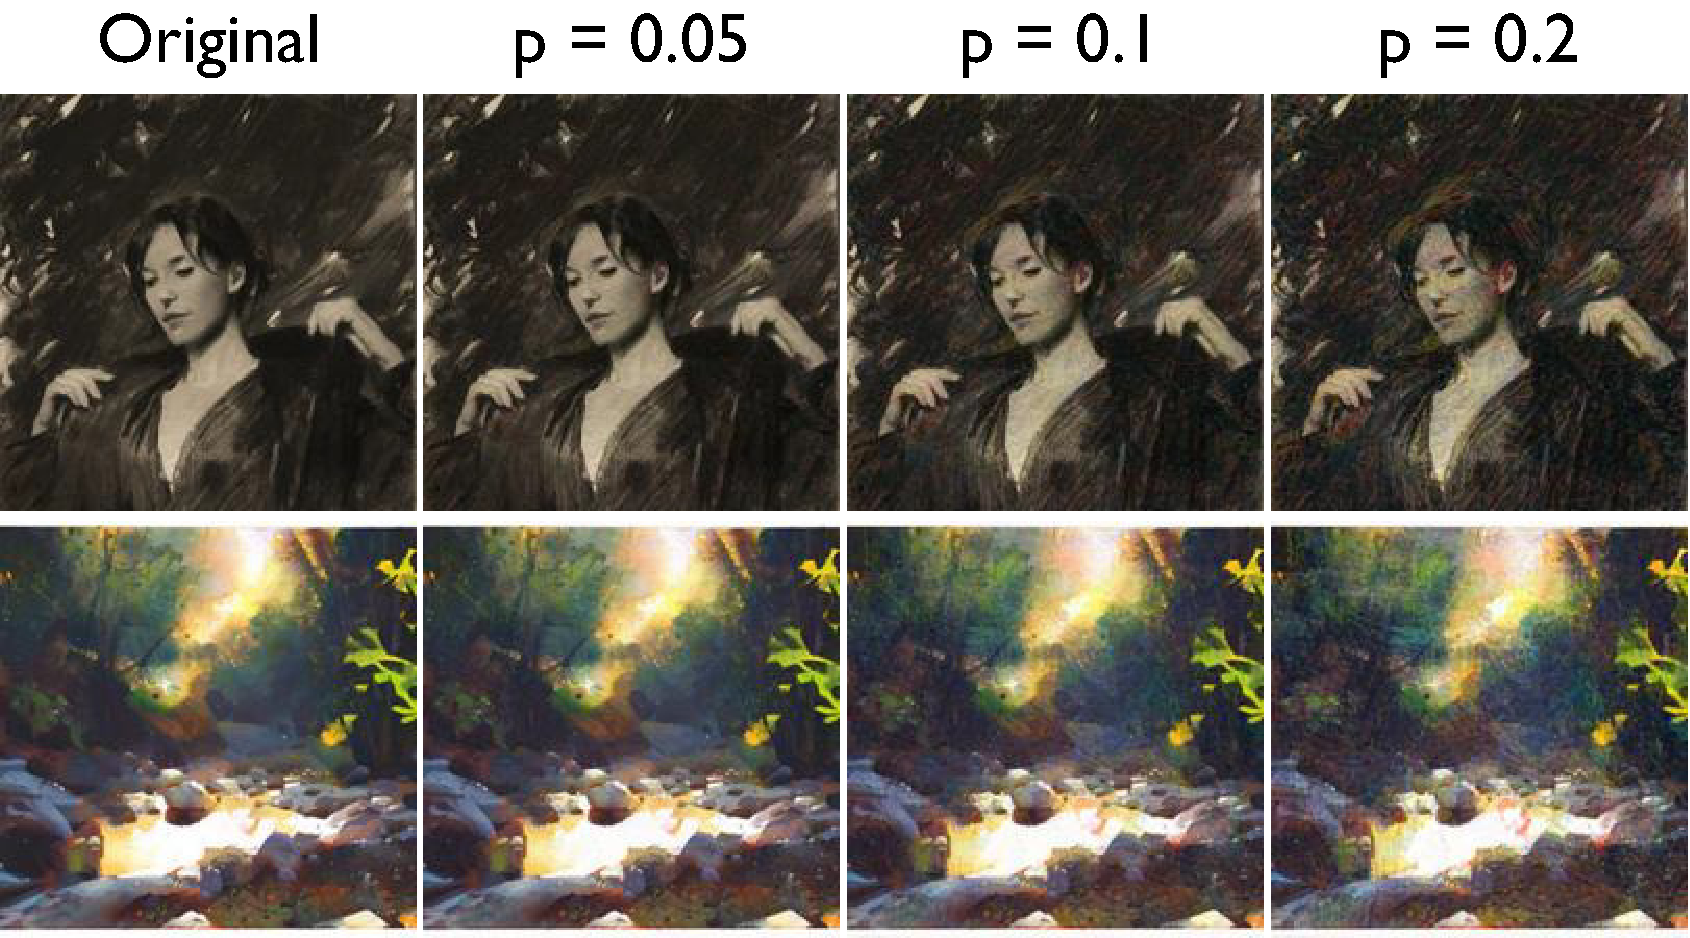
\includegraphics[width=0.90\columnwidth]{plots/eval/cloak-perturbation.pdf}
  \vspace{-0.08in}
  \caption{Original artwork and cloaked artwork computed using three different cloak perturbation budgets. }
  \label{fig:before-after}
\end{figure}

\secspace
\subsection{\system{}'s Protection Performance}
\label{sec:cloaking-results}

\para{Style mimicry success when \system{} is not used. } Mimicry attacks are
very successful when the mimic has access to a victim's original (unmodified)
artwork. Examples of mimicked artwork can be found in
Figure~\ref{fig:core-res}. The leftmost two columns of Figure~\ref{fig:core-res} show a
victim artist's original artwork, while the third column depicts mimicked
artwork generated by a style-specific model trained on victim's original
artwork when \system{} is not used. In our user study, over $>95\%$ of
respondents rated the attack as successful. Table~\ref{tab:psr-core-table},
row 1, gives the artist-rated and CLIP-based genre shift for mimicry attacks on
unprotected art. 

SD models produce stronger mimicry attacks than \dalleM{} models, according
to our user study (see Table~\ref{tab:psr-core-table}). This is unsurprising,
as \dalleM{} models generally produce lower-quality generated
images. CLIP-based genre shift does not reflect this phenomenon, as this metric does
not assess image quality.  

\para{\system{}'s success at preventing style mimicry. } \system{} makes
mimicry attacks markedly less successful, as shown in
Figure~\ref{fig:core-res}. Columns 5 and 6 (from left) show mimicked artwork
when the style-specific models are trained on artwork protected by
\system{}. For reference, column 4 shows an example style-transferred artwork
$\Omega(x, T)$ used to compute \system{} cloaks for the protected art
pieces. Overall, \system{} achieves $> 93.3\%$ artist-rated PSR and
$> 96.0\%$ CLIP-based genre shift (see Table~\ref{tab:psr-core-table}). \system{}'s
protection performance is slightly higher for current artists than for
historical artists. This is likely because the historical artists' images are
present in the training datasets of our generic models (SD, \dalleM),
highlighting the additional challenge of protecting well-known artists whose
style was already learned by the generic models.

\para{How large of perturbations will artists tolerate?} Increasing the
\system{} perturbation budget enhances protection performance. We observe
that both artist-rated and CLIP-based genre shift increase with perturbation budget
(see Figure~\ref{fig:budget-increase}, Table~\ref{tab:budget-increase-sd},
and Figure~\ref{fig:budget2results}). Given this tradeoff between protection
success and \system{} protection visibility on original artwork, we evaluate
how perturbation size impacts artists' willingness to use \system{}. 

We find that artists are willing to add fairly large \system{} perturbations
to their artwork in exchange for protection against mimicry. To measure this,
we show $3$ randomly chosen pairs of original/cloaked artwork to each of the
1,156 artists in our first study. For each art pair, we ask the artist
whether they would be willing to post the cloaked artwork (instead of the
original, unmodified version) on their personal website. More than $92\%$ of
artists select ``willing'' or ``very willing'' when $p=0.05$. This number
only slightly increases to $94.3\%$  when $p=0.03$.
Figure~\ref{fig:artist-accept} details artists' preferences as perturbation
budget increases. (see Figure~\ref{fig:before-after} for examples of cloaked
artwork with increasing $p$). Based on these results, we use perturbation
budget $p = 0.05$ for all our experiments, since most artists are willing to
tolerate this perturbation size.  

Surprisingly, over $32.8\%$ artists are willing to use cloaks with $p=0.2$,
which is clearly visible to human eye (see Figure~\ref{fig:before-after}). While we
are surprised by this high perturbation tolerance, in our follow-up free
response artists noted that they would be willing to tolerate large
perturbations because of the devastating consequence if their styles are
stolen. One participant stated that ``I am willing to sacrifice a bit image
quality for protection.'' Many artists ($>80\%$) also noted that they have
already used traditional, more visually disruptive techniques to protect
their artwork online when posting online, \ie adding watermark or reducing
image resolution. One participant stated that ``I already use low to medium
resolution images only for online posting, thus this would not impact my
quality control too much.'' 

\begin{figure*}[t]
  \centering
  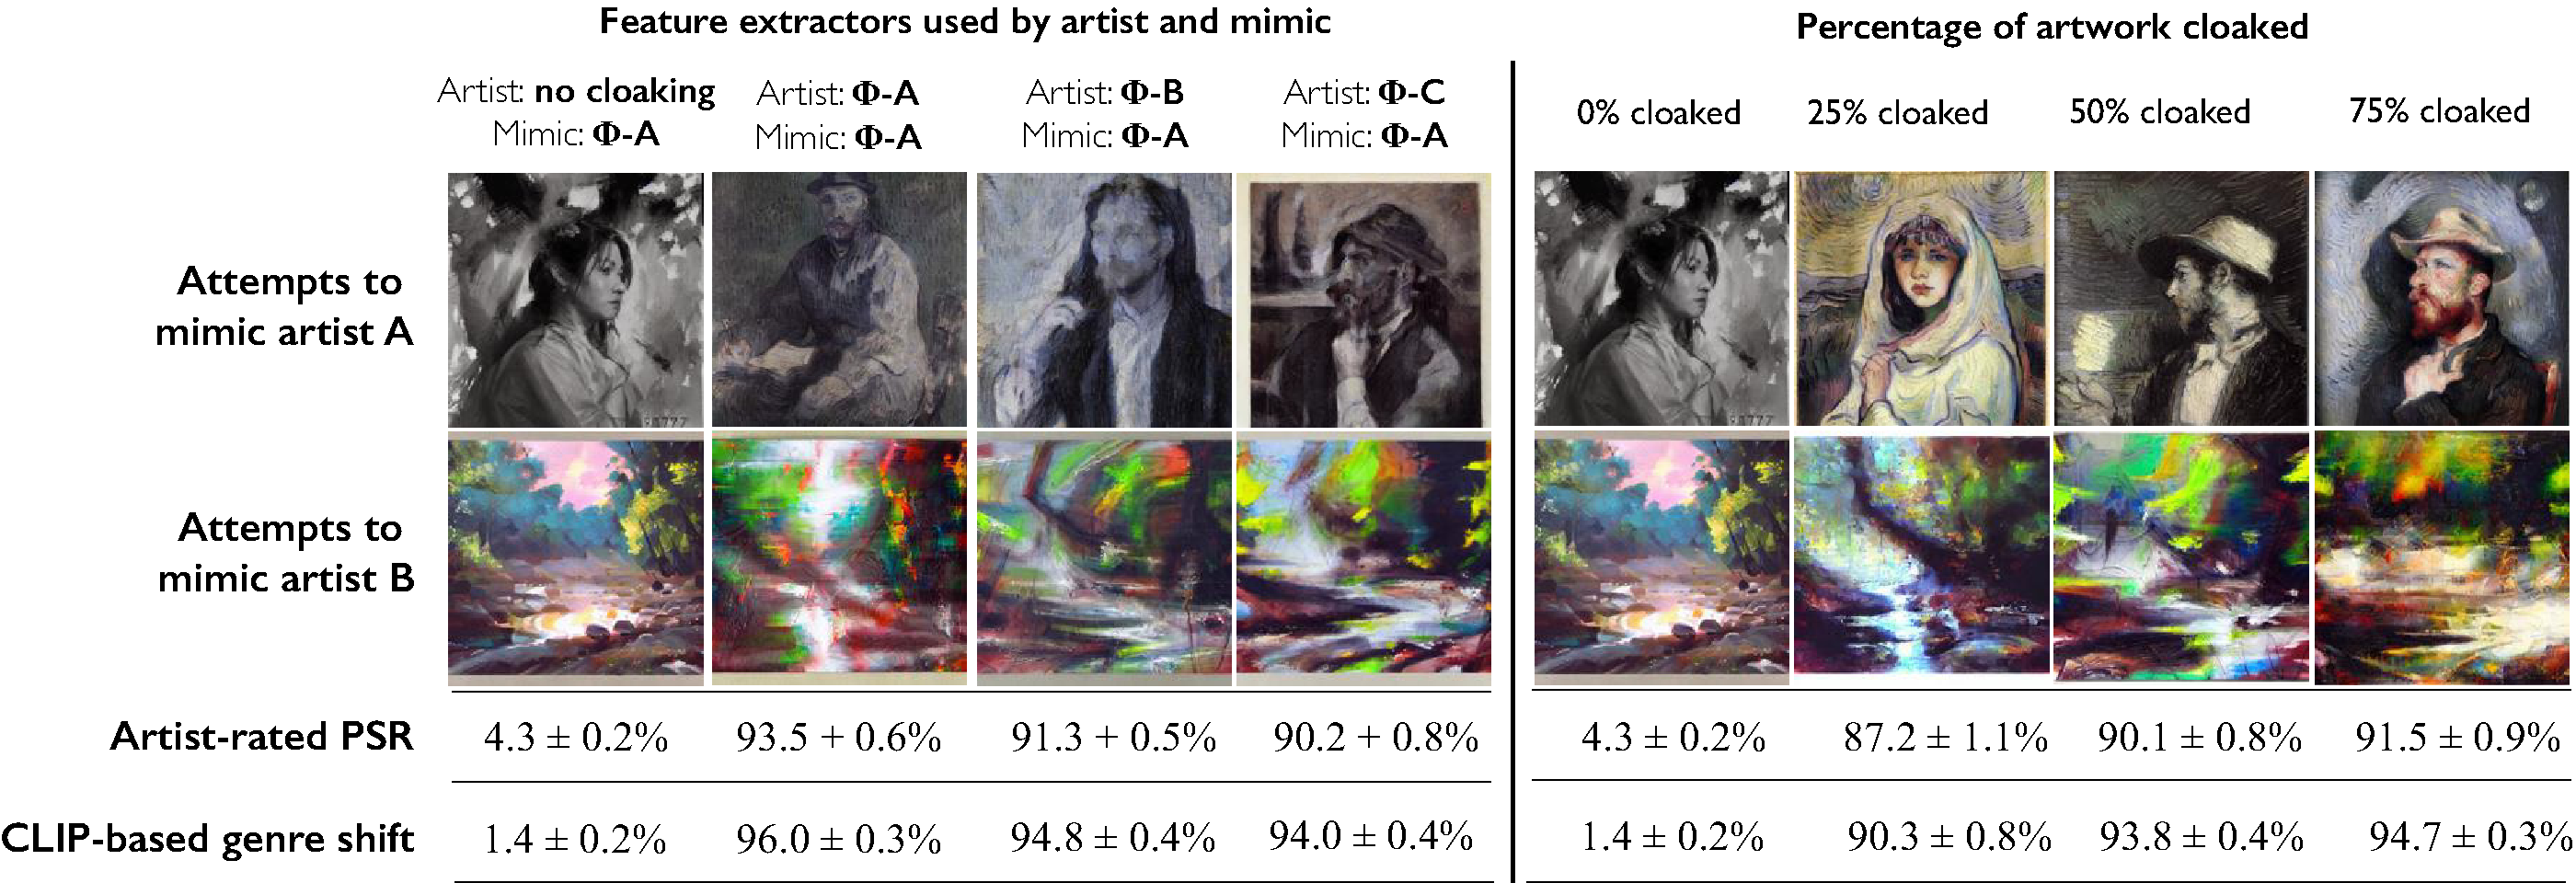
\includegraphics[width=0.95\linewidth]{plots/eval/eval-robust.pdf}
  \caption{\system{} remains successful under two challenging
    scenarios. Left: when artist and mimic use different feature
    extractors. Right: when artists can only cloak a portion of their artwork
    in mimic's dataset. Bottom of the figure shows artist-rated PSR and
    CLIP-based genre shift for the corresponding setting. } 
  \label{fig:core-robust}
\end{figure*}

\secspace
\subsection{\system{}'s Protection Robustness}
\label{sec:robust-eval}

\secspace

Next, we test \system{}'s efficacy in more challenging scenarios. First, we
measure performance when the mimic uses a different feature extractor for
mimicry than the one used by the artist to generate the cloak. Second, we
measure what happens when the mimic has uncloaked artwork samples from the
victim.  Due to the poor mimicry performance of \dalleM, we focus our
evaluation using SD as the generic model.

\para{Artist/mimic use different feature extractors. } In the real world, it
is possible that the mimic will use a different model (and thus a different image
feature extractor) for style mimicry than the one used by the victim artist
to cloak their artwork. While the feature extractors may still be similar
because of the well-known transferability property between large
models~\cite{demontis2019adversarial,transfer,suciu2018does,transfer2014,shan2022post},
their differences could reduce the efficacy of cloaking. We test this
scenario using three feature extractors\textemdash $\Phi$-A, $\Phi$-B, and
$\Phi$-C. $\Phi$-A and $\Phi$-B have different model architectures
(autoencoder-KL~\cite{rombach2022high} vs. VQ-VAE~\cite{ramesh2021zero}) but
are both trained on the ImageNet dataset~\cite{deng2009imagenet}. $\Phi$-A
and $\Phi$-C have different model architectures (autoencoder-KL vs VQ-VAE)
and training datasets (ImageNet vs. CelebA~\cite{liu2018large}).

In our experiments, the victim artist uses one feature extractor (either
$\Phi$-B or $\Phi$-C) to optimize cloaked artwork, and the mimic trains their
style-specific models with SD models using $\Phi$-A. Despite the difference
in victim/mimic extractors, \system{}'s protection remains highly successful
(left half of Figure~\ref{fig:core-robust})\textemdash the style of mimicked
artwork remains distinct from artist's true style. Artist-rated and
CLIP-based genre shift measurements confirm this observation. Artist-rated PSR is
$> 90.2\%$, while CLIP-based genre shift is $> 94.0\%$. The PSR is slightly higher
when the two feature extractors only differ in architectures ($\Phi$-B to
$\Phi$-A) than when they differ in both architecture and training data
($\Phi$-C to $\Phi$-A).


\para{Mimic has access to uncloaked artwork. } Another challenging scenario
is when the mimic gains access to some \textit{uncloaked} artwork from victim
artists. This is a realistic scenario for many prominent artists with a large
online presence. As expected, \system{}'s protection performance decreases
when the mimic has access to more uncloaked artwork (right side of
Figure~\ref{fig:core-robust}). As the ratio of uncloaked/cloaked art in the
mimic's dataset increases, the mimicked artwork becomes more similar to
artist's original style. Yet, \system{} is still reasonably effective
($87.2\%$ artist-rated PSR) even when artists can only cloak $25\%$ of their
artwork. This validates our hypothesis in \S\ref{sec:cloak-effect} that
cloaking will have a noticeable effect as long as the mimic has some cloaked
training data.

A mimic with access to a large amount of uncloaked artwork is still an issue
for \system{}. Fortunately, in our user study, we found that 1) many artists
constantly create and share new artwork online, which can be cloaked to
offset the percentage of uncloaked artwork, and 2) many artists change their
artistic style over time. In our user study, we asked artists to estimate the
number of unique art pieces they currently have online ($M$) and the
estimated number of art pieces they anticipate uploading each subsequent year
($Y$). Among artists with an existing online presence, over $40\%$ have
$Y / M > 25\%$, meaning that one year from now, $> 20\%$ of their total
online artwork would be cloaked (if they start using \system{}
immediately). More than $81\%$ of artists also stated that their art style
has changed over their career, and half of these said that theft of their
old, outdated styles is less concerning.


\begin{table}[t]
  \centering
  \resizebox{0.49\textwidth}{!}{
  \centering
  \begin{tabular}{ccccc}
    \hline
    \multirow{2}{*}{\textbf{\begin{tabular}[c]{@{}c@{}}Artist \\ dataset\end{tabular}}} & \multicolumn{2}{c}{\textbf{w/o \system}} & \multicolumn{2}{c}{\textbf{w/ \system{} (p=0.05)}} \\ \cline{2-5} 
     & \begin{tabular}[c]{@{}c@{}}Artist-rated \\ PSR\end{tabular} & \begin{tabular}[c]{@{}c@{}}CLIP-based \\ genre shift\end{tabular} & \begin{tabular}[c]{@{}c@{}}Artist-rated \\ PSR\end{tabular} & \begin{tabular}[c]{@{}c@{}}CLIP-based \\ genre shift\end{tabular} \\ \hline

    Current & $6.2 \pm 0.5\%$ & $3.8 \pm 0.3\%$ & $92.5 \pm 0.5\%$ & $94.2 + 0.3\%$ \\
    Historical & $7.2 \pm 0.6\%$ & $3.3 \pm 0.4\%$ & $92.1 + 0.3\%$ & $93.9 + 0.4\%$ \\ 
    \hline
    \end{tabular}
  }
  \vspace{-0.1in}
  \caption{Performance of \system{} against real-world mimicry service
    (scenario.gg). Mimicry service achieves high mimicry success when no
    protection is used. When \system{} is used, the mimicry service has low
    performance. }
  \label{tab:real-world}
\end{table}

\secspace
\subsection{Real-World Performance}

Next, we test \system{} against a real-world style mimicry-as-a-service
system, \texttt{scenario.gg}~\cite{aigame}. Scenario.gg is a web service that
allows users to upload a set of images in a specific style. The
service then trains a model to mimic the style and returns an API endpoint
that allows the user to generate mimicked images in the trained style. The
type of model or mimicry method used by the service is unknown.

\system{} remains effective against \texttt{scenario.gg}. We ask
\texttt{scenario.gg} to mimic the style from a set of cloaked or uncloaked
artwork from $4$ current artists and $19$ historical
artists. Table~\ref{tab:real-world} shows that when no protection is used,
\texttt{scenario.gg} can successfully mimic the victim style (< 7.2\%
protection success). The mimicry success of \texttt{scenario.gg} is lower
than our mimicry technique, likely because \texttt{scenario.gg} trains the
model for fewer iterations due to computational constraints. When we use
\system{} to cloak the artwork and upload the cloaked artwork,
\texttt{scenario.gg} fails to mimic the victim style ($> 92.1\%$ artist-rated
PSR and $> 93.9\%$ CLIP-based genre shift rate) as shown in Table~\ref{tab:real-world}.


\section{Ablation Studies}

In this section, we study various aspects of \sys and evaluate the design choices we make with ablation experiments.

\subsection{Kernel Microbenchmark}

The dynamic block mapping in \tech affects the performance of the GPU operations involving the stored KV cache, i.e., block read/writes and attention.
Compared to the existing systems, our GPU kernels (\S\ref{sec:impl}) involve extra overheads of accessing the block table, executing extra branches, and handling variable sequence lengths.
As shown in Fig.~\ref{fig:kernel-latency}, this leads to 20--26\% higher attention kernel latency, compared to the highly-optimized FasterTransformer implementation.
We believe the overhead is small as it only affects the attention operator but not the other operators in the model, such as Linear.
Despite the overhead, \tech makes \sys significantly outperform FasterTransformer in end-to-end performance (\S\ref{sec:eval}).

\begin{figure}[t]
     \centering
     \begin{subfigure}[t]{0.48\linewidth}
         \centering
         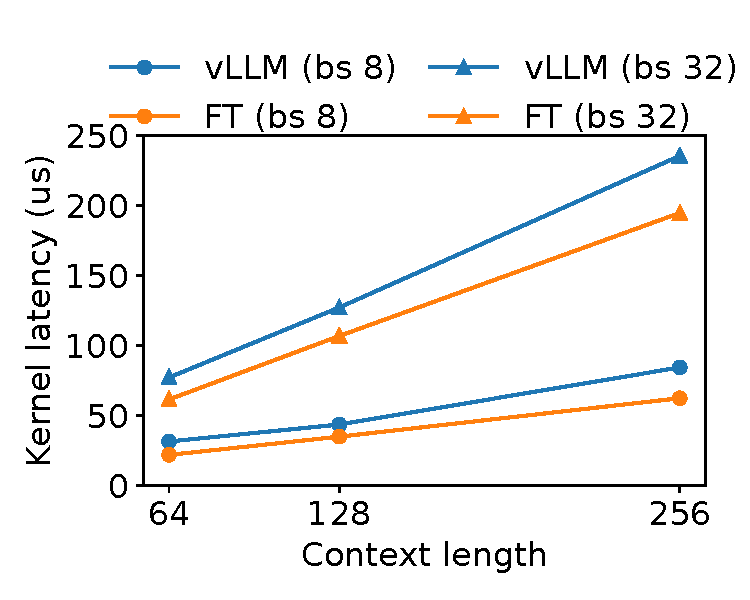
\includegraphics[width=.95\columnwidth]{figures/experiments/micro_latency.pdf}
         \caption{\small Latency of attention kernels.\label{fig:kernel-latency}}
     \end{subfigure}\hfill
     \begin{subfigure}[t]{0.48\linewidth}
         \centering
         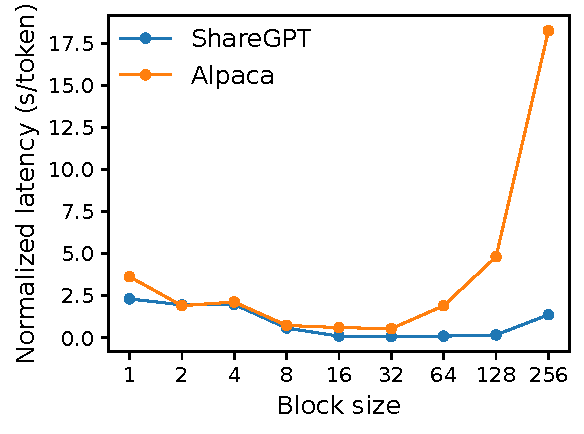
\includegraphics[width=.9\columnwidth]{figures/experiments/n1-block-size.pdf}
         \caption{\small End-to-end latency with different block sizes. \label{fig:block-size-n1}}
     \end{subfigure}
     \vspace{-10pt}
     \caption{Ablation experiments.}
\end{figure}

\subsection{Impact of Block Size}
\label{sec:eval:blocksize}

The choice of block size can have a substantial impact on the performance of \sys.
If the block size is too small, \sys may not fully utilize the GPU's parallelism for reading and processing KV cache.
If the block size is too large, internal fragmentation increases and the probability of sharing decreases.

In Fig.~\ref{fig:block-size-n1}, we evaluate the performance of \sys with different block sizes, using the ShareGPT and Alpaca traces with basic sampling under fixed request rates.
In the ShareGPT trace, block sizes from 16 to 128 lead to the best performance.
In the Alpaca trace, while the block size 16 and 32 work well, larger block sizes significantly degrade the performance since the sequences become shorter than the block sizes.
In practice, we find that the block size 16 is large enough to efficiently utilize the GPU and small enough to avoid significant internal fragmentation in most workloads.
Accordingly, \sys sets its default block size as 16.

\begin{figure}[t]
     \centering
     \begin{subfigure}[t]{0.48\linewidth}
         \centering         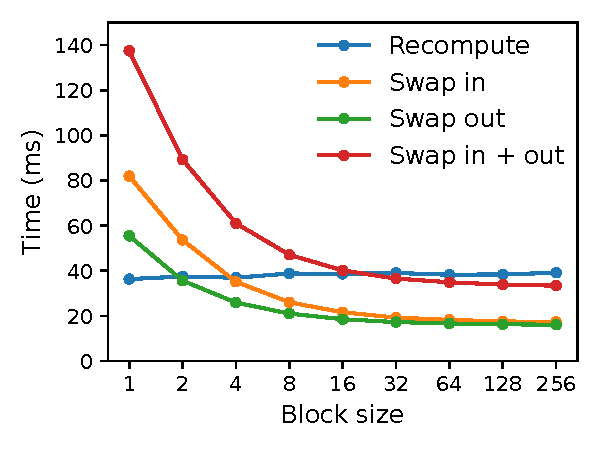
\includegraphics[width=.9\columnwidth]{figures/experiments/micro-swap.pdf}
         \vspace{-7pt}
         \caption{Microbenchmark\label{fig:recomp-vs-swap-micro}}
         
     \end{subfigure}
     \begin{subfigure}[t]{0.48\linewidth}
         \centering        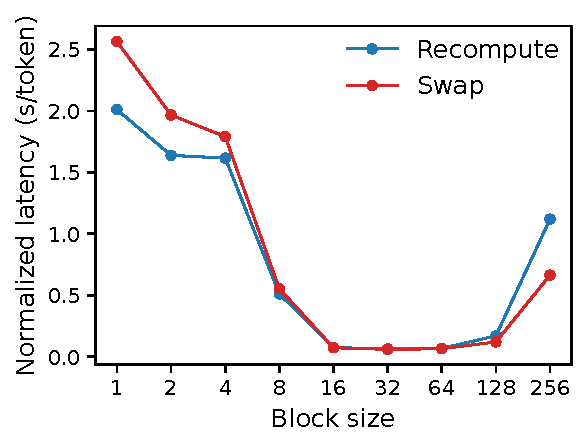
\includegraphics[width=.9\columnwidth]{figures/experiments/recompute-vs-swap.pdf}
         \vspace{-7pt}
         \caption{End-to-end performance\label{fig:recomp-vs-swap-e2e}}
     \end{subfigure}
     \vspace{-3pt}
     \caption{(a) Overhead of recomputation and swapping for different block sizes. (b) Performance when serving OPT-13B with the ShareGPT traces at the same request rate.}
     \vspace{-5pt}
\label{fig:recompute-vs-swap}
\end{figure}

\subsection{Comparing Recomputation and Swapping}
\label{sec:eval:scheduling}

\sys supports both recomputation and swapping as its recovery mechanisms.
To understand the tradeoffs between the two methods, we evaluate their end-to-end performance and microbenchmark their overheads, as presented in Fig.~\ref{fig:recompute-vs-swap}.
Our results reveal that swapping incurs excessive overhead with small block sizes.
This is because small block sizes often result in numerous small data transfers between CPU and GPU, which limits the effective PCIe bandwidth.
In contrast, the overhead of recomputation remains constant across different block sizes, as recomputation does not utilize the KV blocks.
Thus, recomputation is more efficient when the block size is small, while swapping is more efficient when the block size is large, though recomputation overhead is never higher than 20\% of swapping's latency.
For medium block sizes from 16 to 64, the two methods exhibit comparable end-to-end performance.

\section{Discussion}
\label{sec:discussion}

We discuss related work, limitations, and some future directions.

\paragraph{Related Work.}
\cref{sec:discussion:selection} discusses how the selection mechanism relates to similar concepts.
\cref{sec:related} has an extended related work of SSMs and other related models.

\paragraph{No Free Lunch: Continuous-Discrete Spectrum.}
Structured SSMs were originally defined as discretizations of continuous systems \eqref{eq:ssm},
and have had a strong inductive bias toward continuous-time data modalities such as perceptual signals (e.g.\ audio, video).
As discussed in \cref{sec:method:motivation,sec:method:properties}, the selection mechanism overcomes their weaknesses
on discrete modalities such as text and DNA;
but this conversely can impede their performance on data that LTI SSMs excel on.
Our ablations on audio waveforms examine this tradeoff in more detail.

\paragraph{Downstream Affordances.}
Transformer-based foundation models (particularly LLMs) have a rich ecosystem of properties and modes of interaction with pretrained models,
such as fine-tuning, adaptation, prompting, in-context learning, instruction tuning, RLHF, quantization, and so on.
We are particularly interested in whether Transformer alternatives such as SSMs have similar properties and affordances.

%

\paragraph{Scaling.}
Our empirical evaluation is limited to small model sizes,
below the threshold of most strong open source LLMs (e.g. Llama \citep{touvron2023llama})
as well as other recurrent models such as RWKV~\citep{peng2023rwkv} and RetNet~\citep{sun2023retentive},
which have been evaluated at the 7B parameter scale and beyond.
It remains to assess whether Mamba still compares favorably at these larger sizes.
We also note that scaling SSMs may involve further engineering challenges and adjustments to the model
that are not discussed in this paper.

%

%
\section{Related Work}
%


\subsection{Classical Approaches} \label{appendix:related_work_classical}

Classical approaches in time series modeling include the Box-Jenkins method \citep{box1968some}, exponential smoothing  \citep{hyndman2008forecasting, winters1960forecasting}, autoregressive integrated moving average (ARIMA) \citep{box1970time}, and state-space models \citep{hamilton1994state}. In such approaches, the model is usually manually selected based analyzing time series features (e.g., seasonality and order of non-stationarity), where the selected model is then fitted for each individual time series. While classical approaches may be more interpretable than recent deep learning techniques, the domain expertise and manual labor needed to succesfully apply them renders them infeasible to the common setting of modeling thousands, or millions, of time series.

\subsection{Deep Learning Approaches} \label{appendix:related_work_deep}

% (Deep AR, LSTMs, RNNs)
\textbf{Recurrent models.}  Common deep learning architectures for modeling sequence data are the family of recurrent neural networks, which include GRUs~\citep{chung2014empirical}, LSTMs~\citep{hochreiter1997long}, and DeepAR \citep{salinas2020deepar}. However, due to the recurrent nature of RNNs, they are slow to train and may suffer from vanishing/exploding gradients, making them difficult to train \citep{pascanu2013difficulty}. \\

\textbf{Deep State Space models.} Recent work has investigated combining the expressive strengths of SSMs with the scalable strengths of deep neural networks \citep{rangapuram2018, gu2021efficiently}. \cite{rangapuram2018} propose to train a global RNN that transforms input covariates to sequence-spcific SSM parameters; however, one downside of this approach is that they inherit the drawbacks of RNNs. More recent approaches, such as LSSL \citep{gu2021combining}, S4 \citep{gu2021efficiently}, S4D \citep{gu2022parameterization}, and S5 \citep{smith2022simplified}, directly parameterize the layers of a neural network with multiple linear SSMs, and overcome common recurrent training drawbacks by leveraging the convolutional view of SSMs. While deep SSM models have been shown great promise in time series modeling, we show in our work -- which builds off deep SSMs -- that current deep SSM approaches are not able to capture autoregressive processes due to their continuous nature.  \\


\textbf{Neural differential equations as nonlinear state spaces.}
%
\citep{chen2018neural} parametrizes the vector field of continuous--time autonomous systems. These models, termed \textit{Neural Differential Equations} (NDEs) have seen extensive application to time series and sequences, first by \cite{rubanova2019latent} and then by \cite{kidger2020neural,morrill2021neural,massaroli2021differentiable} with the notable extension to \textit{Neural Controlled Differential Equations} (Neural CDEs). Neural CDEs can be considered the continuous--time, nonlinear version of state space models and RNNs \citep{kidger2022neural}. Rather than introducing nonlinearity between linear state space layers, Neural CDEs model nonlinear systems driven by a control input. 

The NDE framework has been further applied by \cite{poli2019graph} to model graph time series via \textit{Neural Graph Differential Equations}. In \cite{queiruga2020continuous}, a continuous-depth ResNet generalization based on ODEs is proposed, and in \cite{kim2021stiff} numerical techniques to enable learning of stiff dynamical systems with Neural ODEs are investigated. The idea of parameterizing the vector field of a differential equation with a neural network, popularized by NDEs, can be traced back to earlier works \citep{funahashi1993approximation, zhang2014comprehensive, weinan2017proposal}. \\



\textbf{Transformers.} 
While RNNs and its variants have shown some success at time series modeling, a major limitation is their applicability to long input sequences. Since RNNs are recurrent by nature, they require long traversal paths to access past inputs, which leads to vanishing/exploding gradients and as a result struggle with capturing long-range dependencies. 

To counteract the long-range dependency problem with RNNs, a recent line of work considers Transformers for time series modeling. The motivation is that due to the attention mechanism, a Transformer can directly model dependencies between any two points in the input sequence, independently of how far apart the points are. However, the high expressivity of the attention mechanism comes at the cost of the time and space complexity being quadratic in sequence length, making Transformers infeasible for very long sequences. As a result, many works consider specialized Transformer architectures with sparse attention mechanisms to bring down the quadratic complexity. For example, \cite{beltagy2020longformer} propose LogSparse self-attention, where a cell attends to a subset of past cells (as opposed to all cells), where closer cells are attended to more frequently, proportional to the log of their distance, which brings down complexity from $\mathcal{O}(\ell^2)$ to $\mathcal{O}(\ell(\log \ell)^2)$. \cite{zhou2021informer} propose ProbSparse self-attention, which achieves $\mathcal{O}(\ell \log \ell)$ time and memory complexity, where they propose a generative style decoder to speed inference. \cite{liu2022pyraformer} propose a pyramidal attention mechanism which shows linear time and space complexity with sequence length. Autoformer \citep{wu2021autoformer} suggests more specialization is needed in time series with a decomposition forecasting architecture, which extracts long-term stationary trend from the seasonal series and utilizes an auto-correlation mechanism, which discovers the period-based dependencies. \cite{zhou2022fedformer} believes previous attempts of Transformer-based architectures do not capture global statistical properties, and to do so requires an attention mechanism in the frequency domain. Confromer \citep{gulati2020conformer} stacks convolutional and self-attention modules into a shared layer to combine the strengths of local interactions from convolutional modules and global interactions from self-attention modules. Perceiver AR \citep{hawthorne2022general} builds on the Perceiver architecture, which reduces the computational complexity of transformers by performing self-attention in a latent space, and extends Perceiver's applicability to causal autoregressive generation.

While these works have shown exciting progress on time series forecasting, their proposed architectures are specialized to handle specific time series settings (e.g., long input sequences, or seasonal sequences), and are commonly trained to output a fixed target horizon length \citep{zhou2021informer}, \ie{} as \emph{direct multi-step forecasting} (DMS) \cite{https://doi.org/10.1111/j.1467-6419.2007.00518.x}. Thus, while effective at specific forecasting tasks, their setups are not obviously applicable to a broad range of time series settings (such as forecasting arbitrary horizon lengths, or generalizing to classification or regression tasks).
%

Moreover, \cite{zeng2022transformers} showed that simpler alternatives to Transformers, such as data normalization plus a single linear layer (NLinear), can outperform these specialized Transformer architectures when similarly trained to predict the entire fixed forecasting horizons. Their results suggest that neither the attention mechanism nor the proposed modifications of these time series Transformers may be best suited for time series modeling. Instead, the success of these prior works  may just be from learning to forecast the entire horizon with fully connected dependencies between prior time-step inputs and future time-step outputs, where a fully connected linear layer is sufficient. \\

\textbf{Other deep learning methods.} Other works also investigate pure deep learning architectures with no explicit temporal components, and show these models can also perform well on time series forecasting. \cite{oreshkin2019n} propose N-BEATS, a deep architecture based on backward and forward residual links. Even simpler, \cite{zeng2022transformers} investigate single linear layer models for time series forecasting. Both works show that simple architectures are capable of achieving high performance for time series forecasting. In particular, with just data normalization, the NLinear model in \cite{zeng2022transformers} obtained state-of-the-art performance on the popular Informer benchmark~\cite{zhou2021informer}. Given an input sequence of past lag terms and a target output sequence of future horizon terms, for every horizon output their model simply learns the fully connected dependencies between that output and every input lag sample. However, FCNs such as NLinear also carry inefficient downsides. Unlike Transformers and SSM-based models, the number of parameters for FCNs scales directly with input and output sequence length, \ie{} $\mathcal{O}(\ell h)$ for $\ell$ inputs and $h$ outputs. Meanwhile, \ourmethod{} shows that the SSM can improve the modeling quality of deep architectures, while maintaining constant parameter count regardless of input or output length. Especially when forecasting long horizons, we achieve higher forecasting accuracy with smaller models.

% \header{S4}\\
\section{Conclusion}
\label{sec:conclusion}
This paper introduced \tool, a language to describe distributed machine learning workloads and optimize them across computation and communication boundary. 
We show that \tool{} generated code significantly improves several training and inference times of large language models. 
In the future we plan to automate the optimizations through smart search.

% With ever increasing larger models being trained on massively
% distributed clusters using large datasets, there is a need for
% optimized communication and computation kernels.  Existing techniques
% to improve data-parallel and model-parallel training are limited to a
% particular algorithm, which might not be optimal for different input
% tensor sizes, topology of a distributed system.  In this paper, we
% presented \tool DSL to express programs that contains communication
% and computation and several transformations to optimize these programs
% for wide range of scenarios.  Code generated by \tool performs
% significantly better than hand-optimized state-of-the-arts.


\section*{Acknowledgement}
We would like to thank Xiaoxuan Liu, Zhifeng Chen, Yanping Huang, anonymous SOSP reviewers, and our shepherd, Lidong Zhou, for their insightful feedback.
This research is partly supported by gifts from Andreessen Horowitz, Anyscale, Astronomer, Google, IBM, Intel, Lacework, Microsoft, Mohamed Bin Zayed University of Artificial Intelligence, Samsung SDS, Uber, and VMware.

\bibliographystyle{ACM-Reference-Format}
\bibliography{reference}


\end{document}
